\documentclass[11pt, a4paper]{article}

% page layout
\usepackage[a4paper, margin=0.77in]{geometry}

% essentials
\usepackage[utf8]{inputenc}
\usepackage[T1]{fontenc}
\usepackage[romanian]{babel}
\usepackage{graphicx}
\usepackage{amsmath}
\usepackage{amssymb}
\usepackage{float}
\usepackage{multicol}

% table enhancements
\usepackage{longtable}
\usepackage{booktabs}
\usepackage{array}

% subfigures
\usepackage{subcaption}

% code listings
\usepackage{xcolor}
\usepackage{listings}

% hyperlinks and document metadata
\usepackage[
    pdftitle={HLTV-DB},
    pdfauthor={Cocu Matei-Iulian},
    pdfsubject={Documentație a bazei de date},
    pdfkeywords={SQL},
    colorlinks=true,
    linkcolor=blue,
    citecolor=red,
    urlcolor=blue
]{hyperref}

\newcommand{\projectname}{Bază de Date Analitică, Istorică (Arhivă) a scenei internaționale de Counter-Strike profesionist}
\newcommand{\dbmsname}{Oracle Database 19c}

% SQL syntax highlighting
\definecolor{codegreen}{rgb}{0,0.6,0}
\definecolor{codegray}{rgb}{0.5,0.5,0.5}
\definecolor{codepurple}{rgb}{0.58,0,0.82}
\definecolor{backcolour}{rgb}{0.95,0.95,0.92}

\lstdefinestyle{sqlstyle}{
    backgroundcolor=\color{backcolour},
    commentstyle=\color{codegreen},
    keywordstyle=\color{magenta},
    numberstyle=\tiny\color{codegray},
    stringstyle=\color{codepurple},
    basicstyle=\ttfamily\footnotesize,
    breakatwhitespace=false,
    breaklines=true,
    captionpos=b,
    keepspaces=true,
    numbers=left,
    numbersep=5pt,
    showspaces=false,
    showstringspaces=false,
    showtabs=false,
    tabsize=2,
    language=SQL
}
\lstset{style=sqlstyle}

\begin{document}

\title{
    Documentație \\
    \large pentru \projectname
}
\author{
    Cocu Matei-Iulian \\
    \small \texttt{matei-iulian.cocu@s.unibuc.ro} \\
    Seria 25, Grupa 252, 2025-2026
}
\date{Versiunea 1.0 \\ \today}
\maketitle

\newpage

\tableofcontents
\newpage

\section{Prezentare}

\textbf{Ce este HLTV} \\
HLTV.org \textit{(Half-Life Television)} reprezintă cea mai vastă arhivă digitală dedicată scenei profesioniste de \textit{Counter-Strike} la nivel global. Platforma funcționează în maniera unui ecosistem complet, oferind știri în timp real, descrierea evenimentelor majore, scoruri live și, esențial, statistici individuale.
\vspace{0.5cm}

\textbf{Scop și Importanță} \\
Se propune proiectarea și implementarea unui model relațional care emulează nucleul operațional al bazei de date HLTV, scopul central fiind gestionarea eficientă a volumului de date generate de ecosistemul E-Sports: de la structura ierarhică a turneelor și logistica meciurilor, până la granularitatea statisticilor individuale. Arhitectura propusă se concentrează exclusiv pe dimensiunea analitică, făcând abstracție de forumul dedicat utilizatorilor. \\ Această bază de date este concepută pentru \dbmsname, folosind Oracle SQL Developer ca mediu de dezvoltare pe Windows ca sistem de operare gazdă.

\section{Descrierea Diagramei Entitate-Relație}
Deoarece modelul propus are ca scop simularea unei platforme analitice complexe pentru E-Sports \textit{(similară HLTV)}, diagrama ER este structurată pe mai multe niveluri de funcționalitate: geografic, administrativ, resurse umane și operațional \textit{(gameplay)}.

\subsection{Entități}

\subsubsection{Entitățile Independente}

\paragraph{Elemente Geografice}
\begin{itemize}
    \item \textbf{REGIUNI}: Reprezintă marile diviziuni geografice competiționale \textit{(ex: EU, NA)}. Este necesară pentru a izola echipele și turneele în funcție de zona de calificare.
    \item \textbf{TARI}: Deși tehnic poate depinde de regiuni, funcționează independent de originea echipelor și a jucătorilor. Atributul cheie este \textit{Codul ISO}, esențial într-o posibilă implementare concretă (afișarea unui steag în interfața grafică).
\end{itemize}

\paragraph{Elemente de Configurare}
\begin{itemize}
    \item \textbf{HARTI}: Definește hărțile de joc disponibile \textit{(ex: Mirage, Nuke)}; este o entitate statică, esențială pentru a lega rundele de contextul spațial.
    \item \textbf{ROLURI}: Standardizează pozițiile tactice \textit{(ex: IGL, Entry, Anchor)}; permite clasificarea jucătorilor și filtrarea statisticilor în funcție de rolul ocupat.
\end{itemize}

\paragraph{Elemente de Business}
\begin{itemize}
    \item \textbf{ORGANIZATORI}: Reprezintă corpurile organizatorice ale turneelor \textit{(ex: ESL, FACEIT, BLAST)}; este o entitate esențială pentru a asocia turneelor o gazdă.
    \item \textbf{SPONSORI}: Reprezintă companiile care oferă suport financiar echipelor participante la diverse competiții \textit{(ex: Red Bull, Razer)}; entitate auxiliară, ce oferă ecosistemului reprezentat o notă de realism.
    \item \textbf{TIPURI\_EVENIMENT}: Standardizează tipurile de evenimente organizate \textit{(ex: Major, Regional LAN, Online)}, fiind esențială granulării nivelului de magnitudine al evenimentului.
\end{itemize}

\subsubsection{Entitățile Dependente și Operaționale}

\paragraph{Ierarhia Resurselor Umane}
\begin{itemize}
    \item \textbf{MEMBRI (Superclasă)}: Centralizează datele comune tuturor persoanelor \textit{(ex: nume, naționalitate, data nașterii)}, eliminând redundanța, depinzând de \textbf{TARI}.
    \item \textbf{JUCATORI (Subclasă)}: Extensie cu atribute specifice performanței active \textit{(ex: rezoluție monitor, setări periferice)}; depinde existențial de \textbf{MEMBRI} și funcțional de \textbf{ROLURI}.
    \item \textbf{ANTRENORI (Subclasă)}: Gestionează personalul tehnic, având atribute specifice stilului de antrenorat.
\end{itemize}

Entitatea Organizațională \textbf{ECHIPE} \\
Reprezintă cluburile profesioniste; este dependentă de \textbf{TARI} \textit{(pentru steagul echipei)} și conține atribute volatile \textit{(ranking mondial)}, care se actualizează dinamic. Bineînțeles, intră în strânsă legătură cu entitatea \textbf{MEMBRI}.

\paragraph{Fluxul Competițional}
\begin{itemize}
    \item \textbf{TURNEE}: Reprezintă evenimentul în sine; depinde de \textbf{ORGANIZATORI} și \\ \textbf{TIPURI\_EVENIMENT}.
    \item \textbf{MECIURI}: Instanța unei confruntări directe între două \textbf{ECHIPE}. Este o entitate dependentă de \textbf{TURNEE}, conținând atribute specifice contextuale \textit{(temporal (DATA\_ORA) și formatul (ex: BO3))}.
    \item \textbf{RUNDE}: Cea mai granulară entitate \textit{temporală}. Depinde de intersecția dintre \textbf{ECHIPE} și \textbf{HARTI}, stocând rezultatul punctual (câștigător, condiție victorie).
\end{itemize}

Entitatea de legătură \textbf{INSTANTE\_MECI\_HARTA} \\
Reprezintă entitatea asociativă dintre \textbf{MECIURI} și \textbf{HARTI}, care rezolvă concret granularitatea unui singur meci disputat. Este esențială pentru a lega \textbf{RUNDE} de contextul spațial și temporal al unei hărți, implicit al unui meci.

\subsection{Relații}

\subsubsection{Relații de Ierarhizare \textit{(Generalizare/Specializare)}}
\textbf{Relația MEMBRI - JUCATORI/ANTRENORI}: Este o relație de tip "Is-A" \textit{(este un)}, totală \textit{(în contextul rolului principal)}, modelând moștenirea atributelor comune; cardinalitatea este \texttt{1(1):1(0)}; la nivel de implementare, un membru poate fi atât jucător, cât și antrenor, chiar și simultan.

\subsubsection{Relații Structurale \textit{(One-to-Many)}}
\begin{itemize}
    \item \textbf{REGIUNI conțin TARI}: O regiune poate conține mai multe țări (sau niciuna, la momentul înregistrării), însă o țară aparține obligatoriu unei singure regiuni \textit{(cardinalitate 1(1):M(0))}.
    \item \textbf{TARI au ca cetățeni MEMBRI}: O țară poate fi originea mai multor membri (sau niciunul, la momentul înregistrării), iar un membru poate avea sau nu o naționalitate \textit{(cardinalitate 1(0):M(0))}.
    \item \textbf{ORGANIZATORI organizează TURNEE}: Un organizator poate gestiona mai multe evenimente (sau niciunul, la momentul înregistrării), însă un turneu este obligatoriu legat de o singură entitate organizatoare \textit{(cardinalitate 1(1):M(0))}.
    \item \textbf{TIPURI\_EVENIMENT clasifică TURNEE}: Un tip de eveniment poate clasifica mai multe turnee (sau niciunul, la momentul înregistrării), însă un turneu este obligatoriu legat de un singur tip de eveniment \textit{(cardinalitate 1(1):M(0))}.
    \item \textbf{TURNEE includ MECIURI}: Un turneu include mai multe meciuri (sau niciunul, la momentul înregistrării sau dacă a fost anulat, de exemplu), iar existența unui meci depinde de existența unui turneu organizat, justificând cardinalitatea \texttt{1(1):M(0)}.
    \item \textbf{ROLURI sunt atribuite la JUCATORI}: Fiind de sine stătător, un rol poate fi atribuit unui jucător (sau niciunuia, la momentul înregistrării acestora), dar unui jucător trebuie să îi fie obligatoriu asignat un rol \textit{(se poate presupune că acesta este Rifler, un rol generic ce poate fi atribuit oricărui jucător de pe scena profesionistă a jocului)}, justificând astfel cardinalitatea \textit{1(1):M(0)}.
    \item \textbf{MECIURI implică INSTANTE\_MECI\_HARTA}: Un meci se desfășoară după un anumit format \textit{(BO1, BO3, BO5)}; astfel, un meci poate avea mai multe instanțe (sau niciuna, la momentul înregistrării sau dacă meciul a fost câștigat la masa verde de o echipă), dar o instanță de meci este obligatoriu asignată unui singur meci, confirmând astfel cardinalitatea \textit(1(1):M(0)).
    \item \textbf{HARTI sunt alese în INSTANTE\_MECI\_HARTA}: O singură hartă poate fi jucată în cadrul mai multor meciuri (sau a niciunuia, la momentul înregistrării), dar dacă există o instanță a unui meci în care a fost aleasă o hartă, atunci acea hartă trebuie să existe, justificând astfel cardinalitatea \textit{1(1):M(0)}.
    \item \textbf{INSTANTE\_MECI\_HARTA se desfășoară pe RUNDE}: O hartă care se dispută în cadrul unui meci se desfășoară pe parcursul a mai multe runde (sau nu, la momentul înregistrării sau dacă meciul, implicit harta, a fost câștigată la masa verde), dar o rundă nu poate exista independent, aceasta este obligatoriu asociată unei instanțe, justificând astfel cardinalitatea \textit{1(1):M(0)}.
\end{itemize}

\subsubsection{Relații de Asociere \textit{(Many-to-Many)}}
\begin{itemize}
    \item \textbf{ECHIPE sponsorizate de SPONSORI}: Modelează fluxul financiar; o echipă poate avea \textit{(sau nu)} contracte simultane cu mai mulți sponsori, iar un sponsor poate finanța \textit{(sau nu)} multiple echipe cardinalitate \textit{(M(0):M(0))}. O echipă poate fi sponsorizată de un sponsor la un anumit moment, fiind esențială mențiunea că o echipă poate fi susținută de mai multe ori de același sponsor, în perioade diferite de timp.
    \item \textbf{ECHIPE au (avut) activi MEMBRI}: O echipă poate avea în selecția acesteia multipli jucători (sau niciunul, la momentul înregistrării acesteia), iar un jucător poate juca în cariera acestuia la mai multe echipe (niciodată simultan). Așadar, mențiunea că un jucător nu poate fi înregistrat sub numele unei organizații de mai multe ori concomitent, dar acesta poate avea mai multe contracte cu respectiva echipă. Astfel, este stabilită o relație de cardinalitate \textit{M(0):M(0)}.
    \item \textbf{JUCATORI au statistici pe RUNDE}: Un jucător are înregistrate statistici pe mai multe runde (sau niciuna, la momentul înregistrării sau dacă acesta este rezervă), iar o rundă înregistrează statisticile a mai mulți jucători (sau a niciunuia, la momentul înregistrării sau alte cazuri speciale), fiind astfel stabilită o relație de cardinalitate \textit{M(0):M(0)}.
\end{itemize}

\section{Diagrama Entitate-Relație (ER)}
\begin{figure}[H]
    \centering
    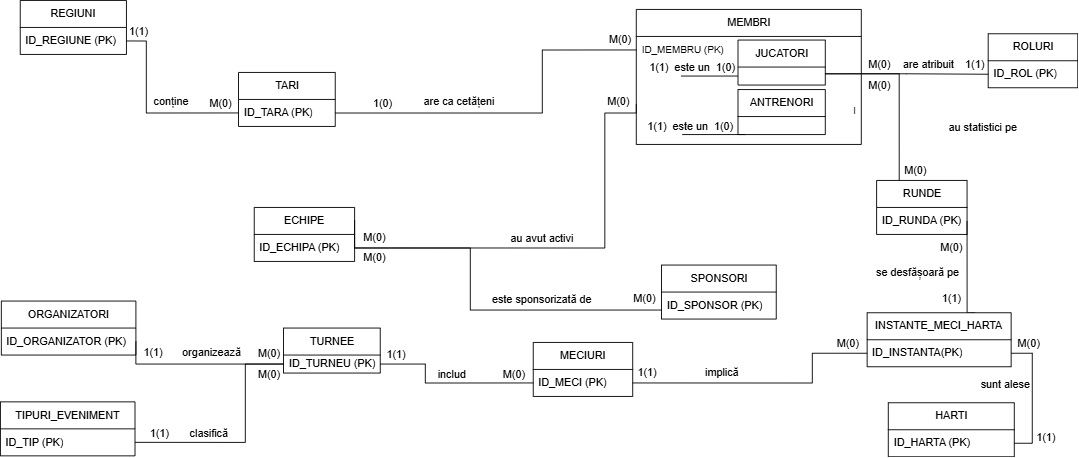
\includegraphics[width=0.93\textwidth]{resources/diagrama_er.png}
    \caption{Diagrama Entitate-Relație a Proiectului}
    \label{fig:diagrama_er}
\end{figure}

\section{Diagrama Conceptuală}
\begin{figure}[!ht]
    \centering
    \makebox[\textwidth][c]{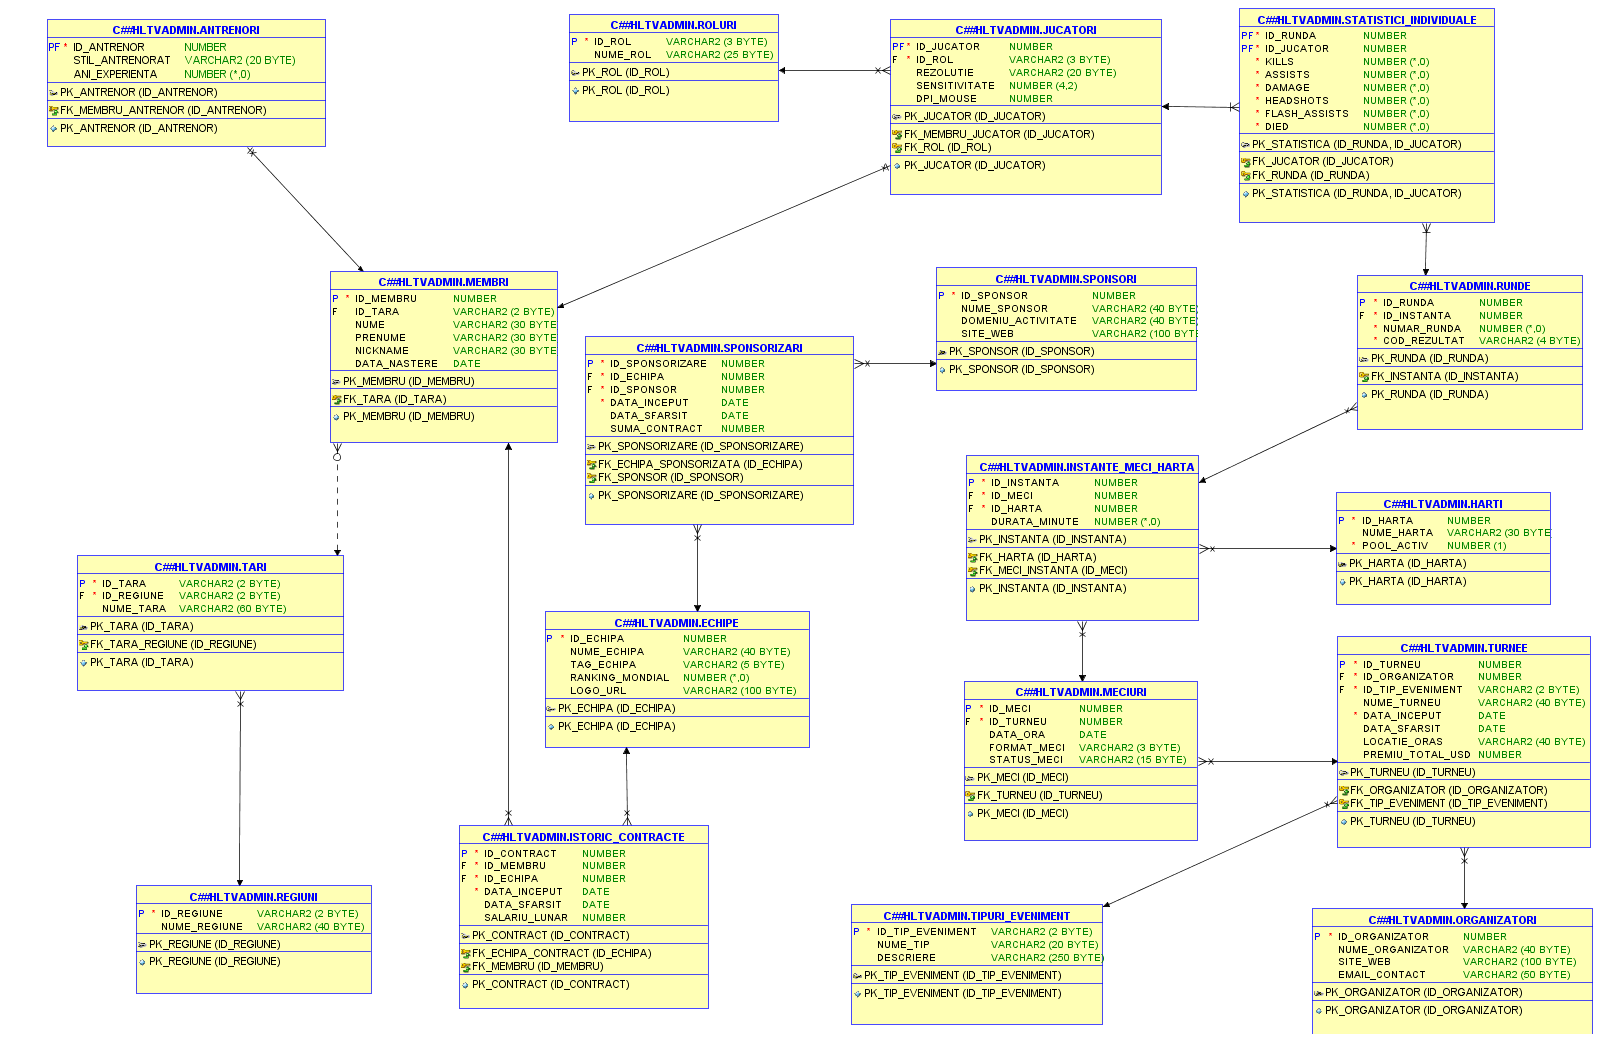
\includegraphics[width=1.23\textwidth]{resources/diagrama_conceptuala.png}}
    \caption{Diagrama Conceptuală a Proiectului}
    \label{fig:diagrama_conceptuala}
\end{figure}

\newpage
\section{Implementarea Diagramei Conceptuale}
\begin{lstlisting}[language=SQL, numbers=none]
CREATE TABLE regiuni (
    id_regiune   VARCHAR2(2),
    nume_regiune VARCHAR2(40),
    
    CONSTRAINT pk_regiune PRIMARY KEY (id_regiune)
);
\end{lstlisting}

\begin{lstlisting}[language=SQL, numbers=none]
CREATE TABLE tari (
    id_tara    VARCHAR2(2),
    id_regiune VARCHAR2(2) NOT NULL,
    nume_tara  VARCHAR2(60),
    
    CONSTRAINT pk_tara PRIMARY KEY (id_tara),
    CONSTRAINT fk_tara_regiune FOREIGN KEY (id_regiune)
        REFERENCES regiuni(id_regiune) ON DELETE CASCADE
);
\end{lstlisting}

\begin{lstlisting}[language=SQL, numbers=none]
CREATE TABLE tipuri_eveniment (
    id_tip_eveniment VARCHAR2(2),
    nume_tip         VARCHAR2(20),
    descriere        VARCHAR2(250),
    
    CONSTRAINT pk_tip_eveniment PRIMARY KEY (id_tip_eveniment)
);
\end{lstlisting}

\begin{lstlisting}[language=SQL, numbers=none]
CREATE TABLE roluri (
    id_rol   VARCHAR2(3),
    nume_rol VARCHAR2(25),
    
    CONSTRAINT pk_rol PRIMARY KEY (id_rol)
);
\end{lstlisting}

\begin{lstlisting}[language=SQL, numbers=none]
CREATE TABLE harti (
    id_harta NUMBER GENERATED BY DEFAULT ON NULL
        AS IDENTITY (START WITH 1 CACHE 20 NOORDER),
    nume_harta VARCHAR2(30),
    pool_activ NUMBER(1) DEFAULT 0 NOT NULL,
    
    CONSTRAINT pk_harta PRIMARY KEY (id_harta),
    CONSTRAINT chk_pool_activ CHECK (pool_activ IN (0, 1))
);
\end{lstlisting}

\begin{lstlisting}[language=SQL, numbers=none]
CREATE TABLE organizatori (
    id_organizator NUMBER GENERATED BY DEFAULT ON NULL
        AS IDENTITY (START WITH 3000 CACHE 20 NOORDER),
    nume_organizator VARCHAR2(40),
    site_web         VARCHAR2(100),
    email_contact    VARCHAR2(50),
    
    CONSTRAINT pk_organizator PRIMARY KEY (id_organizator),
    CONSTRAINT chk_valid_website_org
        CHECK(REGEXP_LIKE(site_web, '^(https?://)?([a-zA-Z0-9.-]+)\.([a-zA-Z]{2,})(/.*)?$')),
    CONSTRAINT chk_valid_email
        CHECK(REGEXP_LIKE(email_contact, '^[A-Za-z0-9._%+-]+@[A-Za-z0-9.-]+\.[A-Za-z]{2,}$'))
);
\end{lstlisting}

\newpage
\begin{lstlisting}[language=SQL, numbers=none]
CREATE TABLE sponsori (
    id_sponsor NUMBER GENERATED BY DEFAULT ON NULL
        AS IDENTITY (START WITH 5000 CACHE 20 NOORDER),
    nume_sponsor       VARCHAR2(40),
    domeniu_activitate VARCHAR2(40),
    site_web           VARCHAR2(100),
    
    CONSTRAINT pk_sponsor PRIMARY KEY (id_sponsor),
    CONSTRAINT chk_valid_website_spn
        CHECK(REGEXP_LIKE(site_web, '^(https?://)?([a-zA-Z0-9.-]+)\.([a-zA-Z]{2,})(/.*)?$'))
);
\end{lstlisting}

\begin{lstlisting}[language=SQL, numbers=none]
CREATE TABLE echipe (
    id_echipa NUMBER GENERATED BY DEFAULT ON NULL
        AS IDENTITY (START WITH 100000 CACHE 20 NOORDER),
    nume_echipa     VARCHAR2(30),
    tag_echipa      VARCHAR2(5),
    ranking_mondial INTEGER,
    logo_url        VARCHAR2(100),
    
    CONSTRAINT pk_echipa PRIMARY KEY (id_echipa),
    CONSTRAINT chk_nume_echipa_valid CHECK (LENGTH(nume_echipa) > 2)
);
\end{lstlisting}

\begin{lstlisting}[language=SQL, numbers=none]
CREATE TABLE turnee (
    id_turneu NUMBER GENERATED BY DEFAULT ON NULL
        AS IDENTITY (START WITH 1 CACHE 20 NOORDER),
    id_organizator   NUMBER NOT NULL,
    id_tip_eveniment VARCHAR2(2) NOT NULL,
    nume_turneu      VARCHAR2(40),
    data_inceput     DATE NOT NULL,
    data_sfarsit     DATE,
    locatie_oras     VARCHAR2(40),
    premiu_total_usd NUMBER,
    
    CONSTRAINT pk_turneu PRIMARY KEY (id_turneu),
    CONSTRAINT fk_organizator FOREIGN KEY (id_organizator)
        REFERENCES organizatori(id_organizator) ON DELETE CASCADE,
    CONSTRAINT fk_tip_eveniment FOREIGN KEY (id_tip_eveniment)
        REFERENCES tipuri_eveniment(id_tip_eveniment) ON DELETE CASCADE,
    CONSTRAINT chk_perioada_valida_turneu CHECK (data_sfarsit >= data_inceput)
);
\end{lstlisting}

\begin{lstlisting}[language=SQL, numbers=none]
CREATE TABLE membri (
    id_membru NUMBER GENERATED BY DEFAULT ON NULL
        AS IDENTITY (START WITH 1 CACHE 20 NOORDER),
    id_tara      VARCHAR2(2),
    nume         VARCHAR2(30),
    prenume      VARCHAR2(30),
    nickname     VARCHAR2(25),
    data_nastere DATE,
    
    CONSTRAINT pk_membru PRIMARY KEY (id_membru),
    CONSTRAINT fk_tara FOREIGN KEY (id_tara)
        REFERENCES tari(id_tara) ON DELETE SET NULL
);
\end{lstlisting}

\newpage
\begin{lstlisting}[language=SQL, numbers=none]
CREATE TABLE jucatori (
    id_jucator NUMBER,
    id_rol        VARCHAR2(3) DEFAULT 'RFL' NOT NULL,
    rezolutie     VARCHAR2(20),
    sensitivitate NUMBER(4, 2),
    dpi_mouse     NUMBER,
    
    CONSTRAINT pk_jucator PRIMARY KEY (id_jucator),
    CONSTRAINT fk_membru_jucator FOREIGN KEY (id_jucator)
        REFERENCES membri(id_membru) ON DELETE CASCADE,
    CONSTRAINT fk_rol FOREIGN KEY (id_rol)
        REFERENCES roluri(id_rol) ON DELETE CASCADE
);
\end{lstlisting}

\begin{lstlisting}[language=SQL, numbers=none]
CREATE TABLE antrenori (
    id_antrenor     NUMBER,
    stil_antrenorat VARCHAR2(20) DEFAULT 'tactical',
    ani_experienta  INTEGER,
    
    CONSTRAINT pk_antrenor PRIMARY KEY (id_antrenor),
    CONSTRAINT fk_membru_antrenor FOREIGN KEY (id_antrenor)
        REFERENCES membri(id_membru) ON DELETE CASCADE
);
\end{lstlisting}

\begin{lstlisting}[language=SQL, numbers=none]
CREATE TABLE sponsorizari (
    id_sponsorizare NUMBER GENERATED BY DEFAULT ON NULL
        AS IDENTITY (START WITH 1 CACHE 20 NOORDER),
    id_echipa     NUMBER NOT NULL,
    id_sponsor    NUMBER NOT NULL,
    data_inceput  DATE NOT NULL,
    data_sfarsit  DATE,
    suma_contract NUMBER,
    
    CONSTRAINT pk_sponsorizare PRIMARY KEY (id_sponsorizare),
    CONSTRAINT fk_echipa_sponsorizata FOREIGN KEY (id_echipa)
        REFERENCES echipe(id_echipa) ON DELETE CASCADE,
    CONSTRAINT fk_sponsor FOREIGN KEY (id_sponsor)
        REFERENCES sponsori(id_sponsor) ON DELETE CASCADE,
    CONSTRAINT chk_perioada_valida_sponsorizare CHECK (data_sfarsit >= data_inceput)
);
\end{lstlisting}

\begin{lstlisting}[language=SQL, numbers=none]
CREATE TABLE istoric_contracte (
    id_contract NUMBER GENERATED BY DEFAULT ON NULL
        AS IDENTITY (START WITH 100 CACHE 20 NOORDER),
    id_membru     NUMBER NOT NULL,
    id_echipa     NUMBER NOT NULL,
    data_inceput  DATE NOT NULL,
    data_sfarsit  DATE,
    salariu_lunar NUMBER,
    
    CONSTRAINT pk_contract PRIMARY KEY (id_contract),
    CONSTRAINT fk_membru FOREIGN KEY (id_membru)
        REFERENCES membri(id_membru) ON DELETE CASCADE,
    CONSTRAINT fk_echipa_contract FOREIGN KEY (id_echipa)
        REFERENCES echipe(id_echipa) ON DELETE CASCADE,
    CONSTRAINT chk_perioada_valida_contract CHECK (data_sfarsit >= data_inceput)
);
\end{lstlisting}

\newpage
\begin{lstlisting}[language=SQL, numbers=none]
CREATE TABLE meciuri (
    id_meci NUMBER GENERATED BY DEFAULT ON NULL
        AS IDENTITY (START WITH 1 CACHE 20 NOORDER),
    id_turneu   NUMBER NOT NULL,
    data_ora    DATE,
    format_meci VARCHAR2(3),

    CONSTRAINT pk_meci PRIMARY KEY (id_meci),
    CONSTRAINT fk_turneu FOREIGN KEY (id_turneu)
        REFERENCES turnee(id_turneu) ON DELETE CASCADE,
    CONSTRAINT chk_format CHECK
        (REGEXP_LIKE(format_meci, '^BO[1,3,5]$', 'i'))
);
\end{lstlisting}

\begin{lstlisting}[language=SQL, numbers=none]
CREATE TABLE instante_meci_harta (
    id_instanta NUMBER GENERATED BY DEFAULT ON NULL
        AS IDENTITY (START WITH 1 CACHE 20 NOORDER),
    id_meci       NUMBER NOT NULL,
    id_harta      NUMBER NOT NULL,
    durata_minute INTEGER,

    CONSTRAINT pk_instanta PRIMARY KEY (id_instanta),
    CONSTRAINT fk_meci_instanta FOREIGN KEY (id_meci)
        REFERENCES meciuri(id_meci) ON DELETE CASCADE,
    CONSTRAINT fk_harta FOREIGN KEY (id_harta)
        REFERENCES harti(id_harta) ON DELETE CASCADE
);
\end{lstlisting}

\begin{lstlisting}[language=SQL, numbers=none]
CREATE TABLE runde (
    id_runda NUMBER GENERATED BY DEFAULT ON NULL
        AS IDENTITY (START WITH 100000 CACHE 20 NOORDER),
    id_instanta  NUMBER NOT NULL,
    numar_runda  INTEGER NOT NULL,
    cod_rezultat VARCHAR2(4) NOT NULL,

    CONSTRAINT pk_runda PRIMARY KEY (id_runda),
    CONSTRAINT fk_instanta FOREIGN KEY (id_instanta)
        REFERENCES instante_meci_harta(id_instanta) ON DELETE CASCADE,
    CONSTRAINT chk_valid_round CHECK (numar_runda > 0),
    CONSTRAINT chk_cod_rezultat CHECK (cod_rezultat IN ('TRCT', 'ELCT', 'ELT', 'BDCT', 'BET'))
);
\end{lstlisting}

\newpage
\begin{lstlisting}[language=SQL, numbers=none]
CREATE TABLE statistici_individuale (
    id_runda      NUMBER NOT NULL,
    id_jucator    NUMBER NOT NULL,
    kills         INTEGER DEFAULT 0 NOT NULL,
    assists       INTEGER DEFAULT 0 NOT NULL,
    damage        INTEGER DEFAULT 0 NOT NULL,
    headshots     INTEGER DEFAULT 0 NOT NULL,
    flash_assists INTEGER DEFAULT 0 NOT NULL,
    died          INTEGER DEFAULT 0 NOT NULL,
    
    CONSTRAINT pk_statistica PRIMARY KEY (id_runda, id_jucator),
    CONSTRAINT fk_runda FOREIGN KEY (id_runda)
        REFERENCES runde(id_runda),
    CONSTRAINT fk_jucator FOREIGN KEY (id_jucator)
        REFERENCES jucatori(id_jucator),
    CONSTRAINT chk_kls CHECK (kills BETWEEN 0 AND 5),
    CONSTRAINT chk_ast CHECK (assists BETWEEN 0 AND 5),
    CONSTRAINT chk_dmg CHECK (damage BETWEEN 0 AND 500),
    CONSTRAINT chk_hss CHECK (headshots BETWEEN 0 AND 5),
    CONSTRAINT chk_fla CHECK (flash_assists BETWEEN 0 AND 5),
    CONSTRAINT chk_ded CHECK (died IN (0, 1))
);
\end{lstlisting}
\begin{figure}[ht]
    \centering
    \begin{subfigure}[b]{0.45\textwidth}
        \centering
        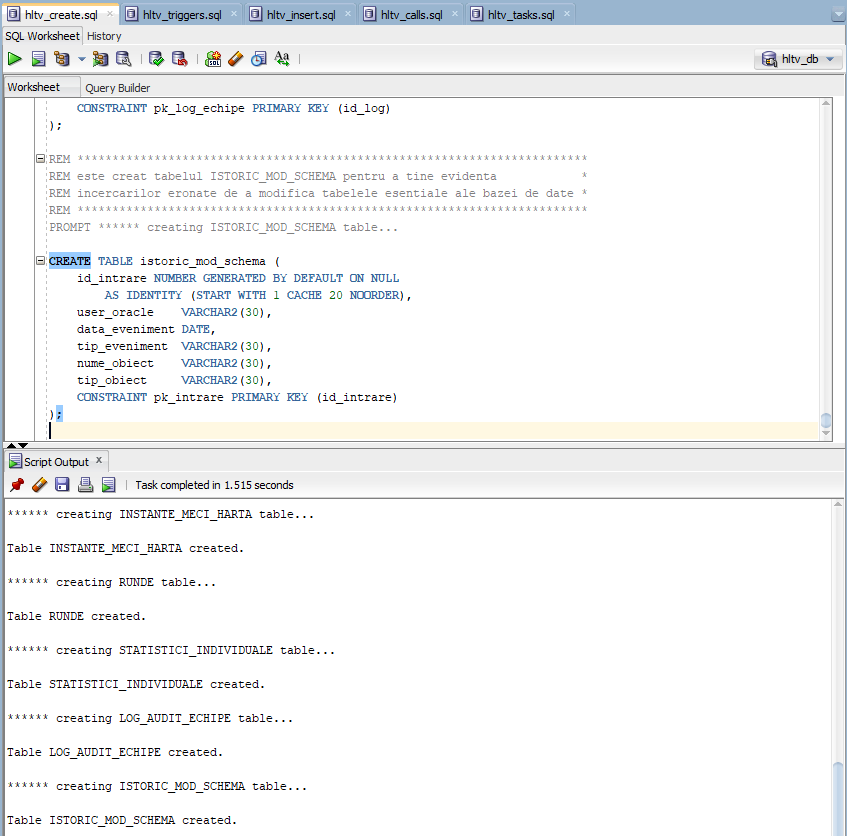
\includegraphics[width=\linewidth]{resources/hltv_create_script.png}
        \label{fig:hltv_create_script}
    \end{subfigure}
    \hfill
    \begin{subfigure}[b]{0.45\textwidth}
        \centering
        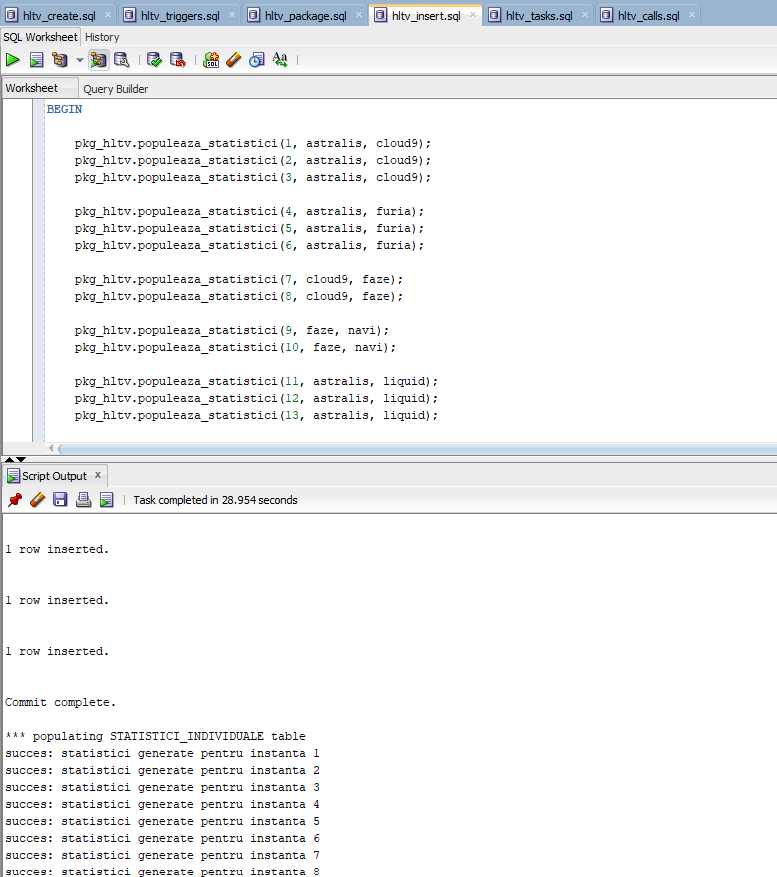
\includegraphics[width=\linewidth]{resources/hltv_insert_script.png}
        \label{fig:hltv_insert_script}
    \end{subfigure}
    \caption{Scripturile de Creare și Inserare Rulate cu Succes}
    \label{fig:shared_scripts_label}
\end{figure}

\newpage
\section{Problema Afișării Celor Mai Buni Jucători}
Se cere să se afișeze topul celor mai buni 10 jucători (după statistici: \textit{average kills per round} \& \textit{average damage per round}) activi care fac parte \textit{de asemenea} din topul celor mai bune 5 echipe din lume.
\begin{lstlisting}[language=SQL, numbers=none]
CREATE OR REPLACE PROCEDURE topul_jucatorilor IS
    TYPE t_info_jucator IS RECORD (
        id_juct jucatori.id_jucator%TYPE,
        nicknam membri.nickname%TYPE,
        nume_ec echipe.nume_echipa%TYPE,
        rank_ec echipe.ranking_mondial%TYPE,
        avg_kls NUMBER,
        avg_dmg NUMBER
    );
    TYPE t_jucatori IS TABLE OF t_info_jucator INDEX BY PLS_INTEGER;
    TYPE t_lista_elita IS TABLE OF t_info_jucator;
    TYPE t_top_varray IS VARRAY(10) OF t_info_jucator;

    v_toti_jucatorii t_jucatori;
    v_lista_elita t_lista_elita := t_lista_elita();
    v_top_final t_top_varray := t_top_varray();
    v_idx PLS_INTEGER;
    v_cnt INTEGER := 0;
    
BEGIN
    DBMS_OUTPUT.PUT_LINE(RPAD('-', 123, '-'));
    DBMS_OUTPUT.PUT_LINE(RPAD('----- sunt selectati toti jucatorii activi', 122) || '|');
    
    FOR r IN (
        SELECT j.id_jucator, m.nickname, e.nume_echipa, e.ranking_mondial,
            ROUND(AVG(s.kills), 2) AS kpr, ROUND(AVG(s.damage), 2) AS adr
        FROM jucatori j
        JOIN membri m ON j.id_jucator = m.id_membru
        JOIN statistici_individuale s ON j.id_jucator = s.id_jucator
        JOIN istoric_contracte i ON m.id_membru = i.id_membru
        JOIN echipe e ON i.id_echipa = e.id_echipa
        WHERE i.data_sfarsit IS NULL
        GROUP BY j.id_jucator, m.nickname, e.nume_echipa, e.ranking_mondial
        ORDER BY kpr DESC, adr DESC
    ) LOOP
        v_toti_jucatorii(r.id_jucator).id_juct := r.id_jucator;
        v_toti_jucatorii(r.id_jucator).nicknam := r.nickname;
        v_toti_jucatorii(r.id_jucator).nume_ec := r.nume_echipa;
        v_toti_jucatorii(r.id_jucator).rank_ec := r.ranking_mondial;
        v_toti_jucatorii(r.id_jucator).avg_kls := r.kpr;
        v_toti_jucatorii(r.id_jucator).avg_dmg := r.adr;
    END LOOP;
    DBMS_OUTPUT.PUT_LINE(RPAD('----- au fost incarcati ' || v_toti_jucatorii.COUNT || ' jucatori activi', 122) || '|');
    DBMS_OUTPUT.PUT_LINE(RPAD('----- sunt filtrati jucatorii din topul 5 mondial al echipelor', 122) || '|');
    
    v_idx := v_toti_jucatorii.FIRST;
    WHILE v_idx IS NOT NULL LOOP
        IF v_toti_jucatorii(v_idx).rank_ec <= 5 THEN
            v_lista_elita.EXTEND;
            v_lista_elita(v_lista_elita.LAST) := v_toti_jucatorii(v_idx);
        END IF;
    
        v_idx := v_toti_jucatorii.NEXT(v_idx);
    END LOOP;
    
    DBMS_OUTPUT.PUT_LINE(RPAD('----- au fost filtrati ' || v_lista_elita.COUNT || ' jucatori', 122) || '|');
    DBMS_OUTPUT.PUT_LINE(RPAD('----- sunt alesi primii 10 jucatori dupa statistici', 122) || '|');
    
    FOR i IN 1..v_lista_elita.COUNT LOOP
        EXIT WHEN v_cnt > 9;
        
        v_top_final.EXTEND;
        v_cnt := v_cnt + 1;
        v_top_final(v_cnt) := v_lista_elita(i);
    END LOOP;
    DBMS_OUTPUT.PUT_LINE(RPAD('-', 123, '-'));
    
    IF v_cnt > 0 THEN
        DBMS_OUTPUT.PUT_LINE('| top | ' || RPAD('nickname', 25) || ' | medie kills runda | medie damage runda | ' ||
        RPAD('nume echipa', 30) || ' | rank global |');
        FOR i IN 1..v_cnt LOOP
            DBMS_OUTPUT.PUT_LINE('| ' || LPAD(TO_CHAR(i), 3) || ' | ' || RPAD(v_top_final(i).nicknam, 25) ||
            ' | ' || RPAD(v_top_final(i).avg_kls, 17) || ' | ' || RPAD(v_top_final(i).avg_dmg, 18) ||
            ' | ' || RPAD(v_top_final(i).nume_ec, 30) || ' | ' || RPAD(v_top_final(i).rank_ec, 11) || ' |');
        END LOOP;
        DBMS_OUTPUT.PUT_LINE(RPAD('-', 123, '-'));
        IF v_cnt < 10 THEN
            DBMS_OUTPUT.PUT_LINE('exista mai putin de 10 jucatori, au fost extrasi toti ' || v_cnt);
        END IF;
    ELSE
        DBMS_OUTPUT.PUT_LINE('----- nu au fost gasite date');
    END IF;
END;
\end{lstlisting}
\begin{figure}[ht]
    \centering
    \begin{subfigure}[b]{0.45\textwidth}
        \centering
        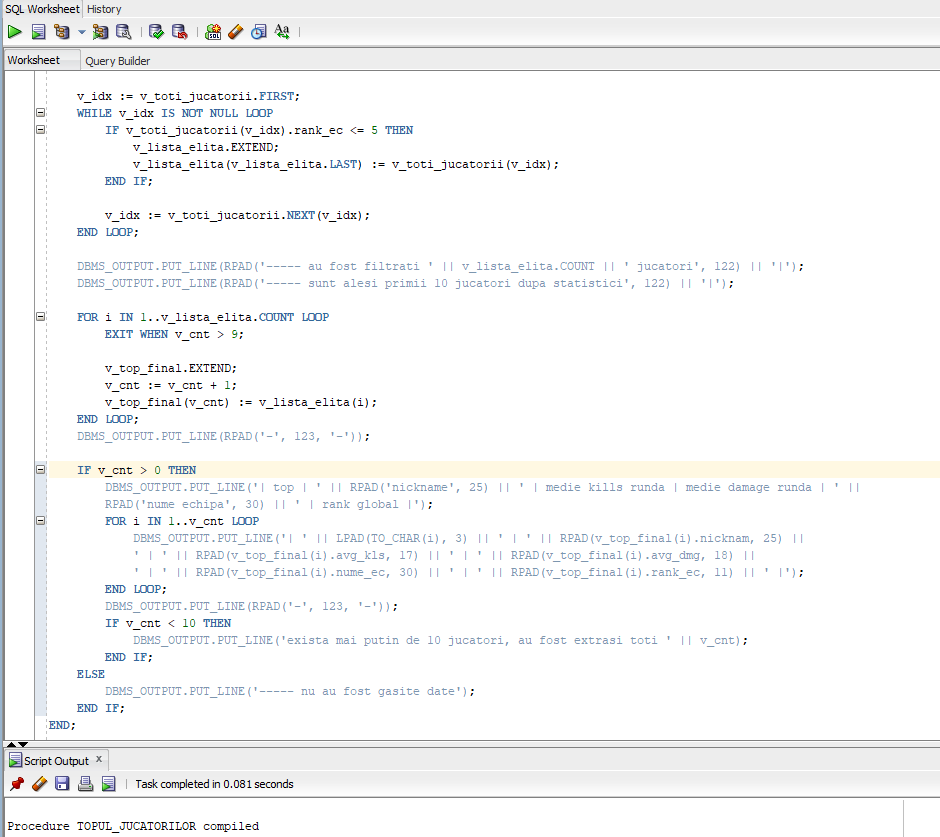
\includegraphics[width=\linewidth]{resources/task6_types.png}
        \label{fig:task6_types}
    \end{subfigure}
    \hfill
    \begin{subfigure}[b]{0.45\textwidth}
        \centering
        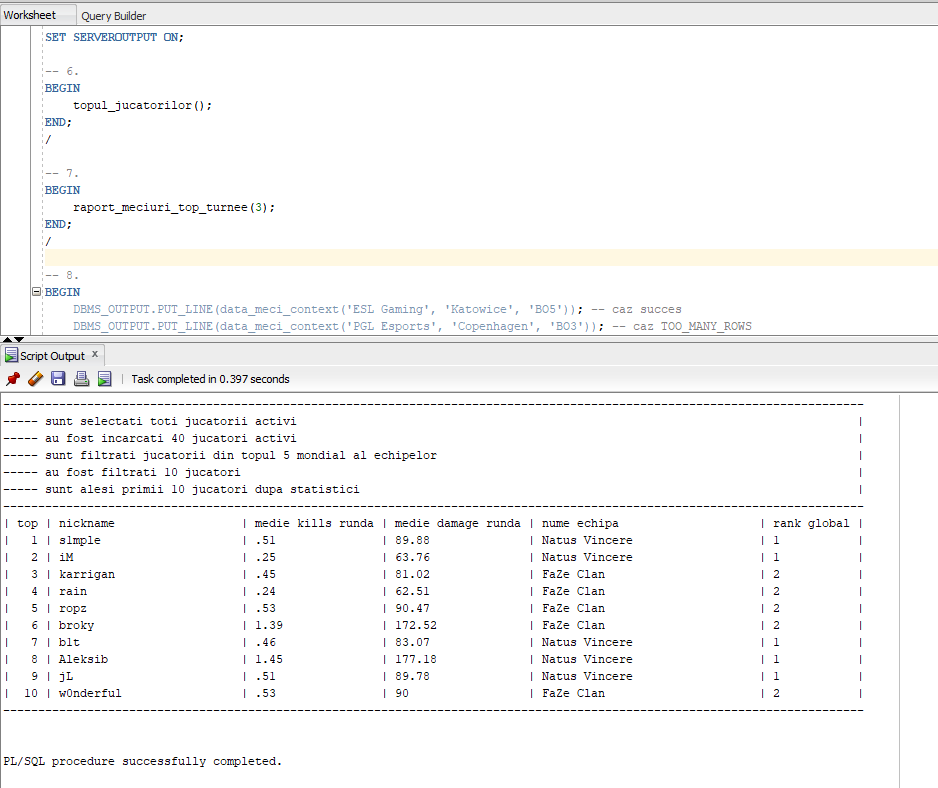
\includegraphics[width=\linewidth]{resources/output_task6.png}
        \label{fig:task6_output}
    \end{subfigure}
    \caption{Sarcina 6 compilată și rulată cu succes}
\end{figure}

\newpage
\section{Problema Celor Mai Importante Turnee}
Dat fiind un număr natural nenul \textbf{n}, se cere să se afișeze primele \textbf{n} turnee organizate după câștiguri, împreună cu informații despre toate meciurile jucate în cadrul acestora \textit{(formatul meciului, data și statutul meciului)}.
\begin{multicols}{2}
\setlength{\columnsep}{1.5cm}
\begin{lstlisting}[language=SQL, numbers=none]
CREATE OR REPLACE PROCEDURE raport_meciuri_top_turnee (
    p_top_n IN INTEGER
) IS
    CURSOR c_meciuri (cp_id_turneu NUMBER) IS
        SELECT data_ora, format_meci
        FROM meciuri
        WHERE id_turneu = cp_id_turneu
        ORDER BY data_ora;

    v_meci_info      c_meciuri%ROWTYPE;
    v_exista_meciuri BOOLEAN;

BEGIN
    DBMS_OUTPUT.PUT_LINE('--- raport top ' || p_top_n || ' turnee (dupa premii) ---');
    
    FOR r IN (
        SELECT id_turneu, nume_turneu, premiu_total_usd, locatie_oras
        FROM turnee
        ORDER BY premiu_total_usd DESC
        FETCH FIRST p_top_n ROWS ONLY
    ) LOOP
        DBMS_OUTPUT.PUT_LINE('------------------------------------------------------');
        DBMS_OUTPUT.PUT_LINE('turneu: ' || r.nume_turneu || ' (premiu: $)' || r.premiu_total_usd || ')');
        DBMS_OUTPUT.PUT_LINE('locatie: ' || r.locatie_oras);
        
        OPEN c_meciuri(r.id_turneu);
        v_exista_meciuri := FALSE;
        
        LOOP
            FETCH c_meciuri INTO v_meci_info;
            EXIT WHEN c_meciuri%NOTFOUND;
            
            v_exista_meciuri := TRUE;
            DBMS_OUTPUT.PUT_LINE('    meci: ' || v_meci_info.format_meci ||
                                ' | data: ' || TO_CHAR(v_meci_info.data_ora, 'DD-MM-YYYY'));
        END LOOP;
            
        IF NOT v_exista_meciuri THEN
            DBMS_OUTPUT.PUT_LINE(' (nu exista meciuri programate pentru acest turneu momentan)');
        END IF;
        CLOSE c_meciuri;
    END LOOP;
END;
\end{lstlisting}
\end{multicols}

\begin{figure}[ht]
    \centering
    \begin{subfigure}[b]{0.45\textwidth}
        \centering
        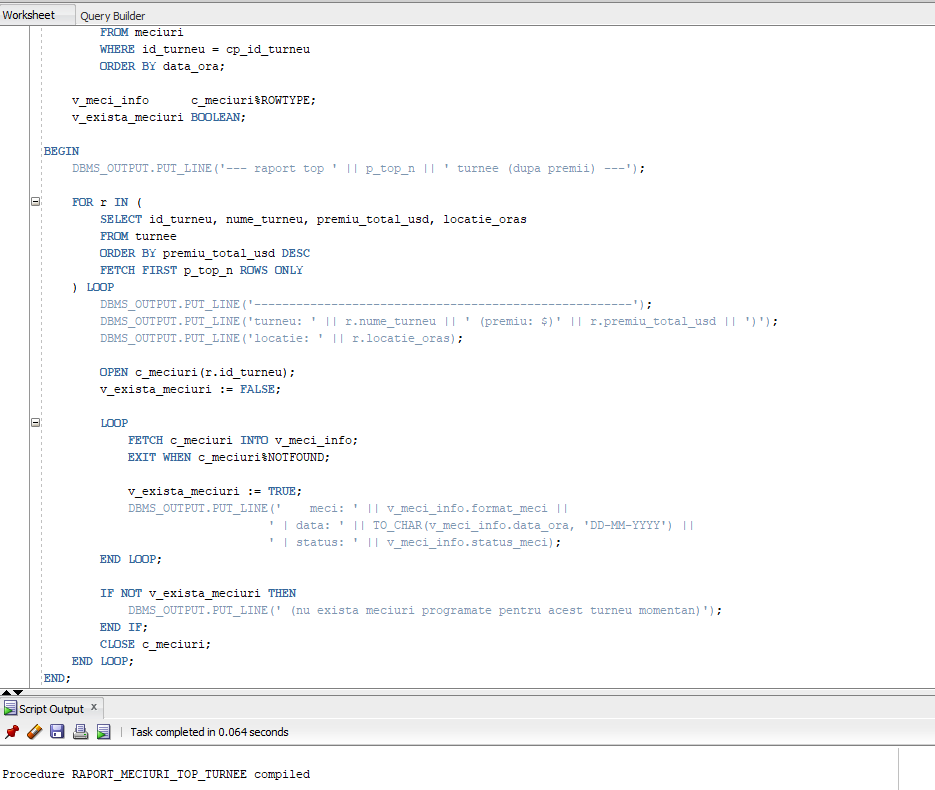
\includegraphics[width=\linewidth]{resources/task7_cursors.png}
        \label{fig:task7_cursors}
    \end{subfigure}
    \hfill
    \begin{subfigure}[b]{0.45\textwidth}
        \centering
        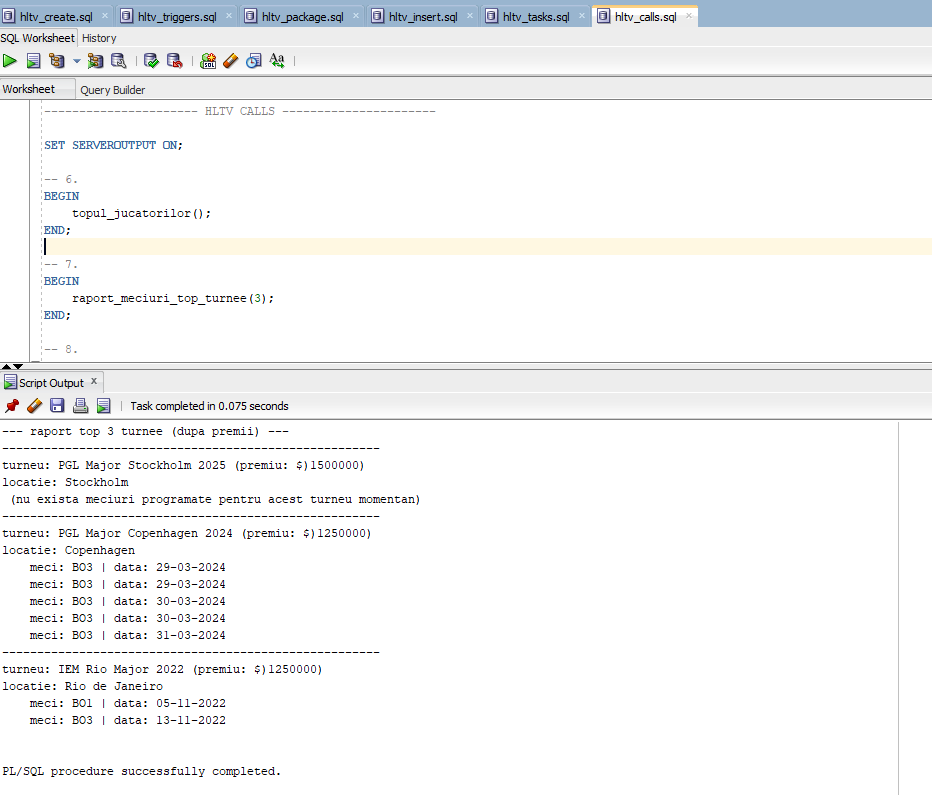
\includegraphics[width=\linewidth]{resources/output_task7.png}
        \label{task7_output}
    \end{subfigure}
    \caption{Sarcina 7 compilată și rulată cu succes}
\end{figure}

\newpage
\section{Problema Meciului Unic}
Date fiind numele unei organizații, un oraș și un format de meci, să se afișeze toate informațiile despre meciul unic jucat în cadrul unui turneu organizat de organizația respectivă în orașul dat, în formatul specificat. Dacă nu există un astfel de meci, să se afișeze un mesaj corespunzător de eroare.
\begin{lstlisting}[language=SQL, numbers=none]
CREATE OR REPLACE FUNCTION data_meci_context (
    p_nume_org IN VARCHAR2,
    p_oras     IN VARCHAR2,
    p_format   IN VARCHAR2
) RETURN VARCHAR2 IS
    v_data_meci DATE;
    v_nume_turneu VARCHAR2(40);
BEGIN
    SELECT m.data_ora, t.nume_turneu
    INTO v_data_meci, v_nume_turneu
    FROM organizatori o
    JOIN turnee t ON o.id_organizator = t.id_organizator
    JOIN meciuri m ON t.id_turneu = m.id_turneu
    WHERE UPPER(o.nume_organizator) = UPPER(p_nume_org)
      AND UPPER(t.locatie_oras) = UPPER(p_oras)
      AND UPPER(m.format_meci) = UPPER(p_format);

    RETURN 'succes: meciul ' || LOWER(p_format) || ' de la ' || LOWER(v_nume_turneu) ||
           ' organizat de ' || LOWER(p_nume_org) || ' a avut loc pe ' || 
           TO_CHAR(v_data_meci, 'DD-MM-YYYY HH24:MI') || ' in orasul ' || LOWER(p_oras);

EXCEPTION
    WHEN NO_DATA_FOUND THEN
        RETURN 'eroare: nu a fost gasit niciun meci ' || LOWER(p_format) ||
               ' pentru ' || LOWER(p_nume_org) || ' in ' || LOWER(p_oras);
        
    WHEN TOO_MANY_ROWS THEN
        RETURN 'eroare: au fost gasite mai multe meciuri ' || LOWER(p_format) ||
               ' pentru ' || LOWER(p_nume_org) || ' in ' || LOWER(p_oras);
        
    WHEN OTHERS THEN
        RETURN 'eroare necunoscuta: ' || SQLCODE || ' - ' || SQLERRM;
END;
\end{lstlisting}
\begin{figure}[ht]
    \centering
    \begin{subfigure}[b]{0.45\textwidth}
        \centering
        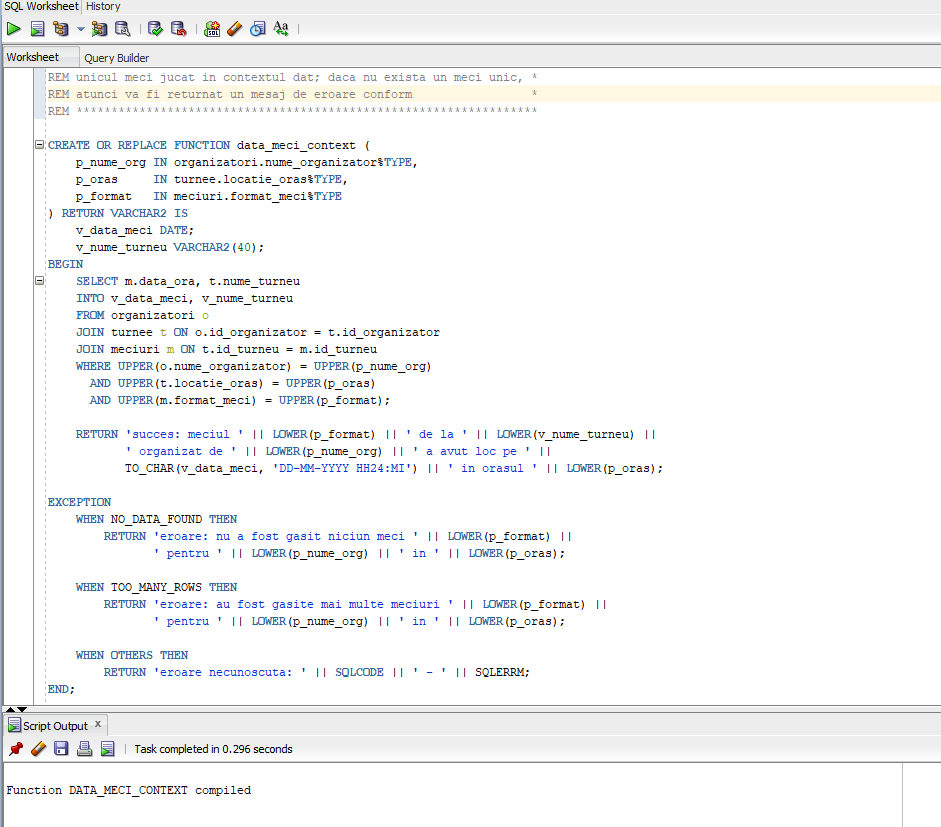
\includegraphics[width=\linewidth]{resources/task8_function.png}
        \label{fig:task8_function}
    \end{subfigure}
    \hfill
    \begin{subfigure}[b]{0.45\textwidth}
        \centering
        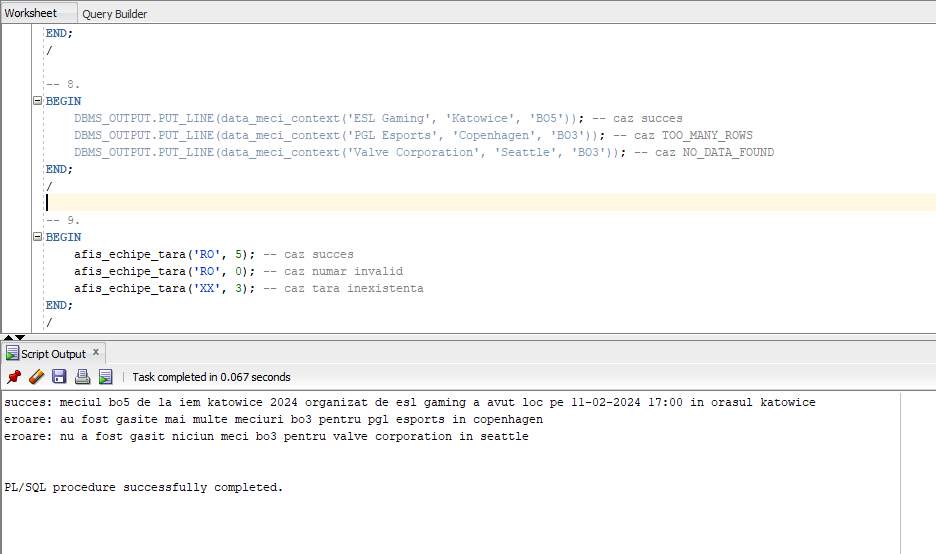
\includegraphics[width=\linewidth]{resources/output_task8.png}
        \label{fig:task8_output}
    \end{subfigure}
    \caption{Sarcina 8 compilată și rulată cu succes}
\end{figure}

\newpage
\section{Problema Naționalităților Echipelor}
Fiind dat un cod ISO al unei țări și un număr natural nenul, să se afișeze datele tuturor echipelor cu cel puțin numărul dat de jucători activi din țara respectivă.
\begin{multicols}{2}
\begin{lstlisting}[language=SQL, numbers=none]
CREATE OR REPLACE PROCEDURE afis_echipe_tara (
    p_id_tara IN tari.id_tara%TYPE,
    p_min_juc IN INTEGER
) IS
    exc_numar_invalid    EXCEPTION;
    exc_tara_inexistenta EXCEPTION;
    
    v_chk_tara NUMBER;
    v_found    BOOLEAN := FALSE;
    v_num_tara tari.nume_tara%TYPE;
BEGIN
    IF p_min_juc <= 0 OR p_min_juc > 5 THEN
        RAISE exc_numar_invalid;
    END IF;

    SELECT COUNT(*) INTO v_chk_tara
    FROM tari
    WHERE UPPER(id_tara) = UPPER(p_id_tara);

    IF v_chk_tara = 0 THEN
        RAISE exc_tara_inexistenta;
    END IF;

    SELECT nume_tara INTO v_num_tara
    FROM tari WHERE id_tara = p_id_tara;

    DBMS_OUTPUT.PUT_LINE('--- raport echipe pentru ' || v_num_tara || ' (minim ' || p_min_juc || ' jucatori) ---');

    FOR r IN (
        SELECT e.nume_echipa, COUNT(j.id_jucator) AS nr_jucatori
        FROM echipe e
        JOIN istoric_contracte i ON e.id_echipa = i.id_echipa
        JOIN membri m ON i.id_membru = m.id_membru
        JOIN jucatori j ON m.id_membru = j.id_jucator
        JOIN tari t ON m.id_tara = t.id_tara
        WHERE i.data_sfarsit IS NULL AND
            UPPER(t.id_tara) = UPPER(p_id_tara)
        GROUP BY e.nume_echipa
        HAVING COUNT(j.id_jucator) >= p_min_juc
        ORDER BY nr_jucatori DESC
    ) LOOP
        v_found := TRUE;
        DBMS_OUTPUT.PUT_LINE('echipa ' || r.nume_echipa || ' cu ' || r.nr_jucatori || ' jucatori');
    END LOOP;

    IF NOT v_found THEN
        DBMS_OUTPUT.PUT_LINE('nicio echipa nu respecta criteriul');
    END IF;

EXCEPTION
    WHEN exc_numar_invalid THEN
        DBMS_OUTPUT.PUT_LINE('eroare utilizator: numarul trebuie sa fie intre 1 si 5.');

    WHEN exc_tara_inexistenta THEN
        DBMS_OUTPUT.PUT_LINE('eroare utilizator: codul iso de tara ' || p_id_tara || ' nu exista');

    WHEN OTHERS THEN
        DBMS_OUTPUT.PUT_LINE('eroare de sistem: ' || SQLCODE || ' - ' || SQLERRM);
END;
\end{lstlisting}
\end{multicols}
\begin{figure}[ht]
    \centering
    \begin{subfigure}[b]{0.35\textwidth}
        \centering
        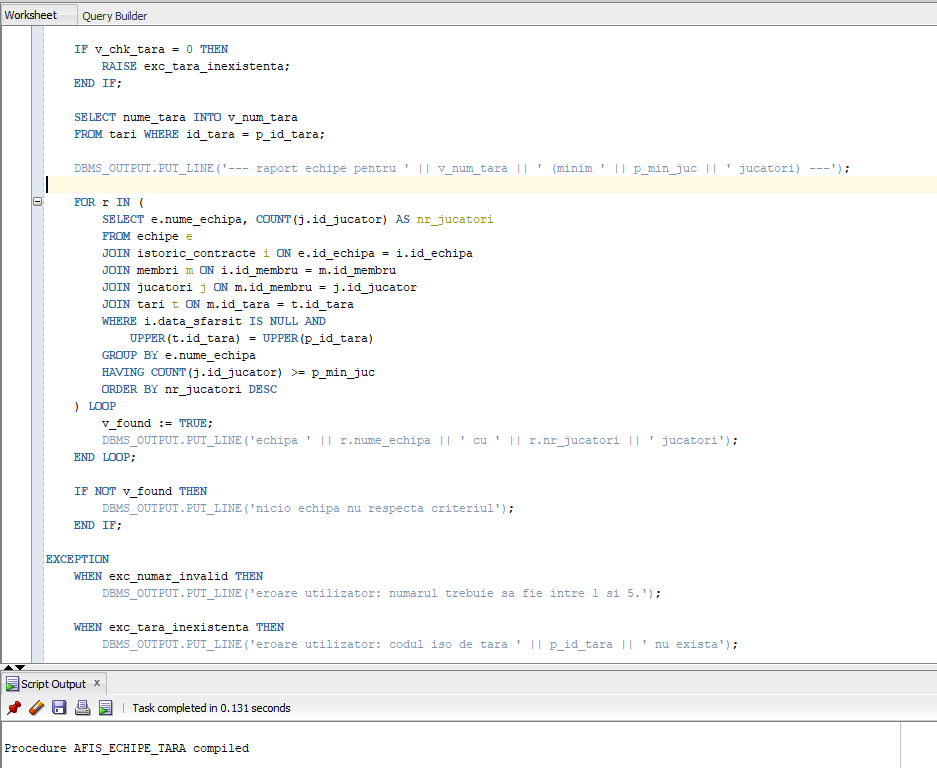
\includegraphics[width=\linewidth]{resources/task9_procedure.png}
        \label{fig:task9_procedure}
    \end{subfigure}
    \hfill
    \begin{subfigure}[b]{0.35\textwidth}
        \centering
        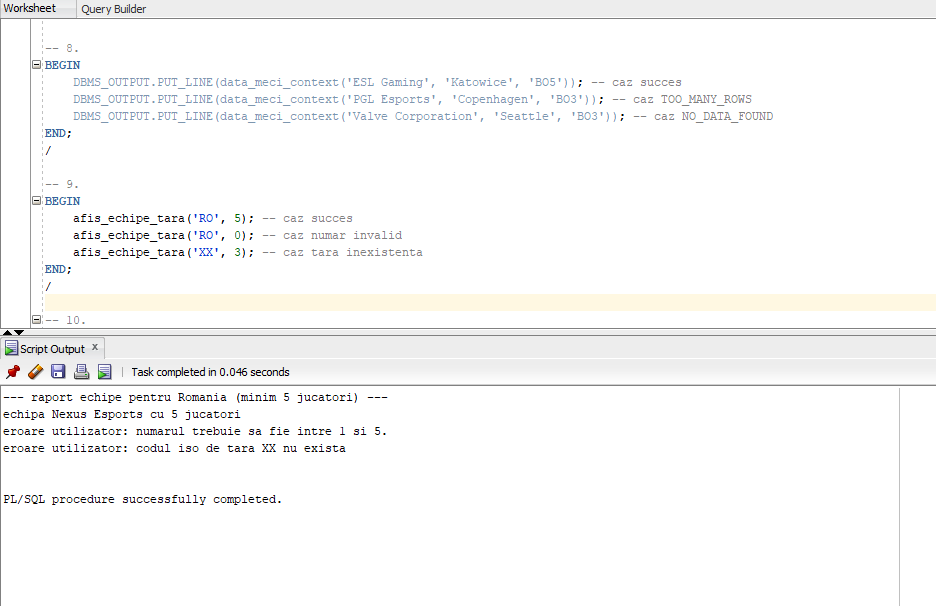
\includegraphics[width=\linewidth]{resources/output_task9.png}
        \label{fig:hltv_output_task9}
    \end{subfigure}
    \caption{\small Sarcina 9 compilată și rulată cu succes}
\end{figure}


\newpage
\section{Auditul Echipelor}
\begin{multicols}{2}
\begin{lstlisting}[language=SQL, numbers=none]
CREATE TABLE log_audit_echipe (
    id_log       NUMBER GENERATED BY DEFAULT AS IDENTITY,
    utilizator   VARCHAR2(50),
    data_actiune DATE,
    tip_operatie VARCHAR2(20),
    
    CONSTRAINT pk_log_echipe PRIMARY KEY (id_log)
);
\end{lstlisting}
\begin{lstlisting}[language=SQL, numbers=none]
REM *** trigger LMD la nivel de comanda *********************
REM sunt inregistrate interventiile asupra tabelului ECHIPE *
REM *********************************************************
CREATE OR REPLACE TRIGGER trg_audit_echipe
AFTER INSERT OR UPDATE OR DELETE ON echipe
DECLARE
    v_tip_op VARCHAR2(20);
BEGIN
    IF INSERTING THEN
        v_tip_op := 'INSERT';
    ELSIF UPDATING THEN
        v_tip_op := 'UPDATE';
    ELSIF DELETING THEN
        v_tip_op := 'DELETE';
    END IF;

    INSERT INTO log_audit_echipe (utilizator, data_actiune, tip_operatie)
    VALUES (USER, SYSDATE, v_tip_op);
END;
\end{lstlisting}
\end{multicols}
\begin{figure}[H]
    \centering
    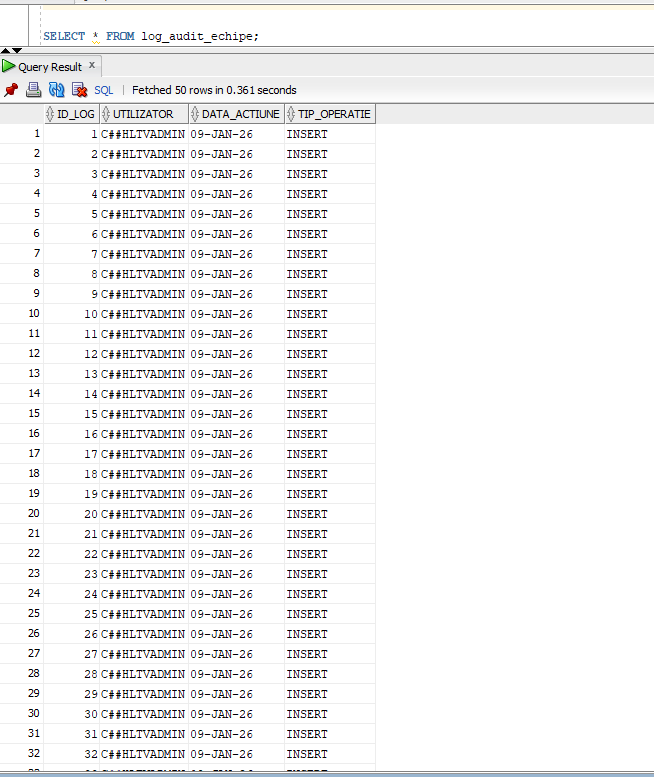
\includegraphics[width=0.75\textwidth]{resources/output_task10.png}
    \caption{Tabelul specific Trigger-ului LMD}
    \label{fig:task10}
\end{figure}

\newpage
\section{Protejarea Schemei}
Adițional, pentru a asigura un anumit nivel de stabilitate a schemei create și a împiedica ștergerea eronată a tabelelor fundamentale, cât și pentru monitorizarea modificărilor tabelelor, este creat un tabel separat \textbf{ISTORIC\_MOD\_SCHEMA}, împreună cu un \textbf{trigger de tip LDD}.
\begin{multicols}{2}
\begin{lstlisting}[language=SQL, numbers=none]
CREATE TABLE istoric_mod_schema (
    id_intrare NUMBER GENERATED BY DEFAULT ON NULL
        AS IDENTITY (START WITH 1 CACHE 20 NOORDER),
    user_oracle    VARCHAR2(30),
    data_eveniment DATE,
    tip_eveniment  VARCHAR2(30),
    nume_obiect    VARCHAR2(30),
    tip_obiect     VARCHAR2(30),
    CONSTRAINT pk_intrare PRIMARY KEY (id_intrare)
);
\end{lstlisting}
\columnbreak
\begin{lstlisting}[language=SQL, numbers=none]
CREATE OR REPLACE TRIGGER trg_protectie_schema
BEFORE DDL ON SCHEMA
DECLARE
    v_operatie  VARCHAR2(30);
    v_obiect    VARCHAR2(30);
    v_tip       VARCHAR2(30);
BEGIN
    v_operatie := ora_sysevent;
    v_obiect   := ora_dict_obj_name;
    v_tip      := ora_dict_obj_type;

    IF v_operatie = 'DROP' AND v_obiect IN ('ECHIPE', 'MEMBRI', 'MECIURI', 'ISTORIC_CONTRACTE') THEN
        RAISE_APPLICATION_ERROR(-20005, 'acces interzis: nu se poate sterge tabelul critic ' || v_obiect);
    END IF;

    INSERT INTO istoric_mod_schema (user_oracle, data_eveniment, tip_eveniment, nume_obiect, tip_obiect)
        VALUES (USER, SYSDATE, v_operatie, v_obiect, v_tip);
END;
\end{lstlisting}
\end{multicols}
\begin{figure}[ht]
    \centering
    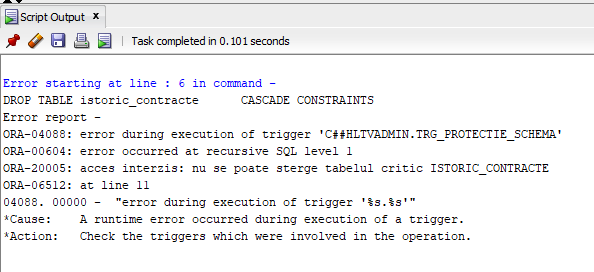
\includegraphics[width=0.9\textwidth]{resources/output_task12.png}
    \caption{Test pentru Trigger-ul LDD}
    \label{fig:task12}
\end{figure}


\newpage
\section{Alți Triggeri Relevanți}
În această secțiune sunt expuse toate obiectele de tip trigger implementate.
\begin{itemize}
    \item \textbf{Verificarea Contractelor unui Membru:} După raționamentul relației de cardinalitate \textit{M(0):M(0)} dintre \textbf{MEMBRI} și \textbf{ECHIPE}, un individ poate face parte dintr-o echipă de mai multe ori, în perioade diferite de timp și poate face parte din mai multe echipe, fără a aparține de mai mult de una singură la un moment dat, astfel fiind explicată motivația din spatele cheii surogate a tabelului asociativ, în defavoarea unei chei primare compuse din cele două chei străine. Așadar, este necesară o verificare externă la modificarea intrărilor existente sau la inserarea a noi intrări în cadrul tabelului \textbf{ISTORIC\_CONTRACTE}.
    \item \textbf{Unicitatea Hărților:} În cadrul unui meci, o anumită hartă nu poate fi jucată decât o singură dată.
    \item \textbf{Respectarea Formatului:} Un meci cu un anumit format nu poate avea mai multe hărți decât numărul indicator indicat; bineînțeles, un meci poate avea mai puține instanțe atribuite acestuia \textit{(un meci BO3 poate avea doar două hărți jucate și să fie terminat, scorul fiind de 2-0, sau dacă meciul este de abia început, atunci scorul poate să fie 0-0)}.
\end{itemize}
\begin{lstlisting}[language=SQL, numbers=none]
REM *** trigger SPONSORIZARI insert **************
REM un sponsor nu poate avea mai multe contracte *
REM care isi suprapun intervalele cu o echipa    *
REM **********************************************

CREATE OR REPLACE TRIGGER trg_sponsorizari_insert
    FOR INSERT ON sponsorizari
    COMPOUND TRIGGER

    TYPE t_linie_noua IS RECORD (
        v_id_echipa  sponsorizari.id_echipa%TYPE,
        v_id_sponsor sponsorizari.id_sponsor%TYPE,
        v_start      DATE,
        v_end        DATE,
        v_rowid      UROWID
    );

    TYPE t_lista_linii IS TABLE OF t_linie_noua INDEX BY PLS_INTEGER;
    v_linii_de_procesat t_lista_linii;
    
    AFTER EACH ROW IS
        v_idx PLS_INTEGER;
    BEGIN
        v_idx := v_linii_de_procesat.COUNT + 1;
        v_linii_de_procesat(v_idx).v_id_echipa  := :NEW.id_echipa;
        v_linii_de_procesat(v_idx).v_id_sponsor := :NEW.id_sponsor;
        v_linii_de_procesat(v_idx).v_start      := :NEW.data_inceput;
        v_linii_de_procesat(v_idx).v_end        := :NEW.data_sfarsit;
        v_linii_de_procesat(v_idx).v_rowid      := :NEW.ROWID;
    END AFTER EACH ROW;

    AFTER STATEMENT IS
        v_cnt NUMBER;
        c_inf CONSTANT DATE := TO_DATE('31-12-9999', 'DD-MM-YYYY');
    BEGIN
        FOR i IN 1..v_linii_de_procesat.COUNT LOOP
            SELECT COUNT(*) INTO v_cnt
            FROM sponsorizari
            WHERE id_echipa = v_linii_de_procesat(i).v_id_echipa
                AND id_sponsor = v_linii_de_procesat(i).v_id_sponsor
                AND ROWID != v_linii_de_procesat(i).v_rowid
                AND v_linii_de_procesat(i).v_start < NVL(data_sfarsit, c_inf)
                AND data_inceput < NVL(v_linii_de_procesat(i).v_end, c_inf);
    
            IF v_cnt > 0 THEN
                RAISE_APPLICATION_ERROR(-20010, 'eroare integritate: exista deja un contract activ sau care se suprapune pentru echipa cu id ' ||
                v_linii_de_procesat(i).v_id_echipa || ' si sponsorul cu id ' || v_linii_de_procesat(i).v_id_sponsor);
            END IF;
        END LOOP;
        
        v_linii_de_procesat.DELETE;
    END AFTER STATEMENT;
END;
/
\end{lstlisting}
\begin{lstlisting}[language=SQL, numbers=none]
REM *** trigger SPONSORIZARI update **************
REM un sponsor nu poate avea mai multe contracte *
REM care isi suprapun intervalele cu o echipa    *
REM data_inceput a sponsorizarii nu se modifica  *
REM data_sfarsit se poate modifica daca e NULL   *
REM **********************************************

CREATE OR REPLACE TRIGGER trg_sponsorizari_update
BEFORE UPDATE OF data_inceput, data_sfarsit ON sponsorizari
FOR EACH ROW
BEGIN
    IF :NEW.data_inceput != :OLD.data_inceput THEN
        RAISE_APPLICATION_ERROR(-20011, 'eroare: nu se poate modifica data de inceput a unei sponsorizari deja salvate');
    END IF;
    
    IF :NEW.data_sfarsit != :OLD.data_sfarsit AND :OLD.data_sfarsit IS NOT NULL THEN
        RAISE_APPLICATION_ERROR(-20012, 'eroare: nu se poate modifica data de sfarsit nenula (' ||
        :OLD.data_sfarsit || ') a unei sponsorizari deja salvate');
    END IF;
    
    IF :NEW.data_sfarsit IS NOT NULL AND :NEW.data_sfarsit < :NEW.data_inceput THEN
        RAISE_APPLICATION_ERROR(-20013, 'eroare: data de sfarsit nu poate fi anterioara datei de inceput');
    END IF;
END;
/
\end{lstlisting}
\begin{lstlisting}[language=SQL, numbers=none]
REM *** trigger ISTORIC_CONTRACTE insert *******************
REM un membru nu poate avea decat un singur contract activ *
REM ********************************************************

CREATE OR REPLACE TRIGGER trg_istoric_contracte_insert
    FOR INSERT ON istoric_contracte
    COMPOUND TRIGGER
    
    TYPE t_linie_noua IS RECORD (
        v_id_membru istoric_contracte.id_membru%TYPE,
        v_id_echipa istoric_contracte.id_echipa%TYPE,
        v_start     DATE,
        v_end       DATE,
        v_rowid     UROWID
    );
    
    TYPE t_lista_linii IS TABLE OF t_linie_noua INDEX BY PLS_INTEGER;
    v_linii_de_procesat t_lista_linii;

    AFTER EACH ROW IS
        v_idx PLS_INTEGER;
    BEGIN
        v_idx := v_linii_de_procesat.COUNT + 1;
        v_linii_de_procesat(v_idx).v_id_membru := :NEW.id_membru;
        v_linii_de_procesat(v_idx).v_id_echipa := :NEW.id_echipa;
        v_linii_de_procesat(v_idx).v_start     := :NEW.data_inceput;
        v_linii_de_procesat(v_idx).v_end       := :NEW.data_sfarsit;
        v_linii_de_procesat(v_idx).v_rowid     := :NEW.ROWID;
    END AFTER EACH ROW;
    
    AFTER STATEMENT IS
        v_cnt NUMBER;
        c_inf CONSTANT DATE := TO_DATE('31-12-9999', 'DD-MM-YYYY');
    BEGIN
        FOR i IN 1..v_linii_de_procesat.COUNT LOOP
            SELECT COUNT(*) INTO v_cnt
            FROM istoric_contracte
            WHERE id_membru = v_linii_de_procesat(i).v_id_membru
                AND ROWID != v_linii_de_procesat(i).v_rowid
                AND v_linii_de_procesat(i).v_start < NVL(data_sfarsit, c_inf)
                AND data_inceput < NVL(v_linii_de_procesat(i).v_end, c_inf);
            
            IF v_cnt > 0 THEN
                RAISE_APPLICATION_ERROR(-20014, 'eroare contract: jucatorul cu id ' || v_linii_de_procesat(i).v_id_membru ||
                ' are deja un contract activ cu echipa ' || v_linii_de_procesat(i).v_id_echipa ||
                ' care se suprapune cu perioada selectata (' || TO_CHAR(v_linii_de_procesat(i).v_start) || ')');
            END IF;
        END LOOP;
    
        v_linii_de_procesat.DELETE;
    END AFTER STATEMENT;
END;
/
\end{lstlisting}
\begin{lstlisting}[language=SQL, numbers=none]
REM *** trigger ISTORIC_CONTRACTE update *******************
REM un membru nu poate avea decat un singur contract activ *
REM data_inceput a sponsorizarii nu se modifica            *
REM data_sfarsit se poate modifica daca e NULL             *
REM ********************************************************

CREATE OR REPLACE TRIGGER trg_istoric_contracte_update
BEFORE UPDATE OF data_inceput, data_sfarsit ON istoric_contracte 
FOR EACH ROW
BEGIN
    IF :NEW.data_inceput != :OLD.data_inceput THEN
        RAISE_APPLICATION_ERROR(-20015, 'eroare: nu se poate modifica data de inceput a unui contract deja salvat');
    END IF;
    
    IF :NEW.data_sfarsit != :OLD.data_sfarsit AND :OLD.data_sfarsit IS NOT NULL THEN
        RAISE_APPLICATION_ERROR(-20016, 'eroare: nu se poate modifica data de sfarsit nenula (' ||
        :OLD.data_sfarsit || ') a unui contract deja salvat');
    END IF;
    
    IF :NEW.data_sfarsit IS NOT NULL AND :NEW.data_sfarsit < :NEW.data_inceput THEN
        RAISE_APPLICATION_ERROR(-20013, 'eroare: data de sfarsit nu poate fi anterioara datei de inceput');
    END IF;
END;
/
\end{lstlisting}
\begin{lstlisting}[language=SQL, numbers=none]
REM *** trigger TURNEE - MECIURI insert *********************
REM un meci nu poate avea data in care a fost jucat in      *
REM afara perioadei desfasurarii turneului de care apartine *
REM *********************************************************

CREATE OR REPLACE TRIGGER trg_turnee_meciuri_insert
BEFORE INSERT OR UPDATE ON meciuri
FOR EACH ROW
DECLARE
    v_data_start DATE;
    v_data_final DATE;
BEGIN
    IF :NEW.data_ora IS NOT NULL AND (
        INSERTING OR
        (:NEW.data_ora != :OLD.data_ora) OR
        (:NEW.id_turneu != :OLD.id_turneu)
    ) THEN
        SELECT data_inceput, data_sfarsit
        INTO v_data_start, v_data_final
        FROM turnee
        WHERE id_turneu = :NEW.id_turneu;
        
        IF :NEW.data_ora < TRUNC(v_data_start) OR :NEW.data_ora >= (v_data_final + 1) THEN
            RAISE_APPLICATION_ERROR(-20014, 'eroare: data meciului (' || TO_CHAR(:NEW.data_ora, 'DD-MM-YYYY') ||
            ') este in afara perioadei turneului (' || TO_CHAR(v_data_start, 'DD-MM-YYYY') || ' - ' ||
            TO_CHAR(v_data_final, 'DD-MM-YYYY') || ')');
        END IF;
    END IF;
EXCEPTION
    WHEN NO_DATA_FOUND THEN
        RAISE_APPLICATION_ERROR(-20015, 'eroare: turneul asociat acestui meci nu a fost gasit');
END;
/
\end{lstlisting}
\begin{lstlisting}[language=SQL, numbers=none]
REM *** trigger TURNEE - MECIURI update *********************
REM un meci nu poate avea data in care a fost jucat in      *
REM afara perioadei desfasurarii turneului de care apartine *
REM sunt mutate toate meciurile afectate la noua data       *
REM *********************************************************

CREATE OR REPLACE TRIGGER trg_turnee_meciuri_update
AFTER UPDATE OF data_inceput, data_sfarsit ON turnee
FOR EACH ROW
BEGIN
    IF :NEW.data_inceput > :OLD.data_inceput THEN
        UPDATE MECIURI
        SET data_ora = :NEW.data_inceput
        WHERE id_turneu = :NEW.id_turneu
            AND data_ora < :NEW.data_inceput;
        
        DBMS_OUTPUT.PUT_LINE('avertisment: data de inceput a turneului a fost modificata, si implicit toate meciurile afectate au fost mutate pe ' || :NEW.data_inceput);
    END IF;

    IF :NEW.data_sfarsit < :OLD.data_sfarsit THEN
        UPDATE MECIURI
        SET data_ora = :NEW.data_sfarsit
        WHERE id_turneu = :NEW.id_turneu
            AND data_ora > :NEW.data_sfarsit;

        DBMS_OUTPUT.PUT_LINE('avertisment: data de sfarsit a turneului a fost modificata, si implicit toate meciurile afectate au fost mutate pe ' || :NEW.data_sfarsit);
    END IF;
END;
/
\end{lstlisting}
\begin{lstlisting}[language=SQL, numbers=none]
REM *** trigger MECIURI - INSTANTE_MECI_HARTA insert **************
REM respectarea formatului meciului: un meci cu un anumit format  *
REM nu poate avea mai multe harti decat numarul indicator asignat *
REM ***************************************************************

CREATE OR REPLACE TRIGGER trg_meciuri_instante_insert
BEFORE INSERT ON instante_meci_harta
FOR EACH ROW
DECLARE
    v_format   meciuri.format_meci%TYPE;
    v_cnt    NUMBER;
    v_max_maps NUMBER;
BEGIN
    SELECT format_meci INTO v_format
    FROM meciuri
    WHERE id_meci = :NEW.id_meci;
    
    IF v_format = 'BO1' THEN v_max_maps := 1;
    ELSIF v_format = 'BO3' THEN v_max_maps := 3;
    ELSIF v_format = 'BO5' THEN v_max_maps := 5;
    ELSE v_max_maps := 1;
    END IF;
    
    SELECT COUNT(*) INTO v_cnt
    FROM instante_meci_harta
    WHERE id_meci = :NEW.id_meci;
    
    IF v_cnt >= v_max_maps THEN
        RAISE_APPLICATION_ERROR(-20016, 'eroare: nu se pot adauga mai multe harti, meciul are format ' || v_format);
    END IF;
END;
/
\end{lstlisting}
\begin{lstlisting}[language=SQL, numbers=none]
REM *** trigger MECIURI - INSTANTE_MECI_HARTA update **************
REM respectarea formatului meciului: un meci cu un anumit format  *
REM nu poate avea mai multe harti decat numarul indicator asignat *
REM nu se poate modifica atributul format_meci al unei intrari    *
REM ***************************************************************

CREATE OR REPLACE TRIGGER trg_meciuri_instante_update
BEFORE UPDATE OF format_meci ON meciuri
FOR EACH ROW
BEGIN
    IF :NEW.format_meci != :OLD.format_meci THEN
        RAISE_APPLICATION_ERROR(-20017, 'eroare: nu se poate modifica formatul unui meci deja salvat');
    END IF;
END;
/

REM *** trigger HARTI - INSTANTE_MECI_HARTA insert ***********
REM unicitatea hartii intr-un meci: o anumita harta nu poate *
REM fi jucata decat o singura data in cadrul unui meci       *
REM **********************************************************

CREATE OR REPLACE TRIGGER trg_harti_instante_insert
    FOR INSERT ON instante_meci_harta
    COMPOUND TRIGGER
    
    TYPE t_linie_noua IS RECORD (
        v_id_meci  instante_meci_harta.id_meci%TYPE,
        v_id_harta instante_meci_harta.id_harta%TYPE,
        v_rowid    UROWID
    );
    
    TYPE t_lista_linii IS TABLE OF t_linie_noua INDEX BY PLS_INTEGER;
    v_linii_de_procesat t_lista_linii;
    
    AFTER EACH ROW IS
        v_idx PLS_INTEGER;
    BEGIN
        v_idx := v_linii_de_procesat.COUNT + 1;
        v_linii_de_procesat(v_idx).v_id_meci  := :NEW.id_meci;
        v_linii_de_procesat(v_idx).v_id_harta := :NEW.id_harta;
        v_linii_de_procesat(v_idx).v_rowid    := :NEW.ROWID;
    END AFTER EACH ROW;

    AFTER STATEMENT IS
        v_cnt NUMBER;
    BEGIN
        FOR i IN 1..v_linii_de_procesat.COUNT LOOP
            SELECT COUNT(*) INTO v_cnt
            FROM instante_meci_harta
            WHERE id_meci = v_linii_de_procesat(i).v_id_meci
                AND id_harta = v_linii_de_procesat(i).v_id_harta
                AND ROWID != v_linii_de_procesat(i).v_rowid;
                
            IF v_cnt > 0 THEN
                RAISE_APPLICATION_ERROR(-20018, 'eroare unicitate: harta cu id ' || v_linii_de_procesat(i).v_id_harta ||
                ' este deja jucata in meciul ' || v_linii_de_procesat(i).v_id_meci);
            END IF;
        END LOOP;
        
        v_linii_de_procesat.DELETE;
    END AFTER STATEMENT;
END;
/
\end{lstlisting}
\begin{lstlisting}[language=SQL, numbers=none]
REM *** trigger HARTI - INSTANTE_MECI_HARTA update ***********
REM unicitatea hartii intr-un meci: o anumita harta nu poate *
REM fi jucata decat o singura data in cadrul unui meci       *
REM cheia straina harta a unei instante nu se poate modifica *
REM **********************************************************

CREATE OR REPLACE TRIGGER trg_harti_instante_update
BEFORE UPDATE OF id_harta ON instante_meci_harta
FOR EACH ROW
BEGIN
    IF :NEW.id_harta != :OLD.id_harta THEN
        RAISE_APPLICATION_ERROR(-20019, 'eroare: nu se poate modifica harta unei instante deja salvate');
    END IF;
END;
/
\end{lstlisting}
\begin{lstlisting}[language=SQL, numbers=none]
REM *** trigger INSTANTE_MECI_HARTA timing ************
REM nu se pot introduce detalii despre desfasurarea   *
REM unui meci inainte ca meciul sa fi inceput oficial *
REM ***************************************************

CREATE OR REPLACE TRIGGER trg_instante_meci_timing
BEFORE INSERT ON instante_meci_harta
FOR EACH ROW
DECLARE
    v_data_meci DATE;
BEGIN
    SELECT data_ora INTO v_data_meci
    FROM meciuri
    WHERE id_meci = :NEW.id_meci;

    IF v_data_meci IS NOT NULL THEN
        IF SYSDATE < v_data_meci THEN
            RAISE_APPLICATION_ERROR(-20020, 
                'eroare cronologica: nu se pot introduce date pentru meciul ' || :NEW.id_meci || 
                ', fiind programat pe ' || TO_CHAR(v_data_meci, 'DD-MM-YYYY HH24:MI') || 
                ', iar acum este ' || TO_CHAR(SYSDATE, 'DD-MM-YYYY HH24:MI'));
        END IF;
    END IF;

EXCEPTION
    WHEN NO_DATA_FOUND THEN
        RAISE_APPLICATION_ERROR(-20021, 'Eroare: Meciul asociat nu exista.');
END;
/
\end{lstlisting}
\begin{lstlisting}[language=SQL, numbers=none]
REM *** trigger STATISTICI_INDIVIDUALE insert ************
REM in cadrul unei runde, ar trebui sa existe statistici *
REM cumulate doar de la maxim 2 echipe, iar fiecare      *
REM echipa sa aiba maxim 5 intrari diferite de jucatori  *
REM ******************************************************

CREATE OR REPLACE TRIGGER trg_statistici_individuale_insert
    FOR INSERT ON statistici_individuale
    COMPOUND TRIGGER
    
    TYPE t_linie_noua IS RECORD (
        v_id_runda   statistici_individuale.id_runda%TYPE,
        v_id_jucator statistici_individuale.id_jucator%TYPE,
        v_rowid      UROWID
    );
    
    TYPE t_lista_linii IS TABLE OF t_linie_noua INDEX BY PLS_INTEGER;
    v_linii_de_procesat t_lista_linii;
    
    AFTER EACH ROW IS
        v_idx PLS_INTEGER;
    BEGIN
        v_idx := v_linii_de_procesat.COUNT + 1;
        v_linii_de_procesat(v_idx).v_id_runda   := :NEW.id_runda;
        v_linii_de_procesat(v_idx).v_id_jucator := :NEW.id_jucator;
        v_linii_de_procesat(v_idx).v_rowid      := :NEW.ROWID;
    END AFTER EACH ROW;
    
    AFTER STATEMENT IS
        c_inf CONSTANT DATE := TO_DATE('31-12-9999', 'DD-MM-YYYY');
        v_id_echipa_curenta NUMBER;
        v_cnt_echipe        NUMBER;
        v_cnt_jucatori      NUMBER;
        v_data_meci         DATE;
    BEGIN
        FOR i IN 1..v_linii_de_procesat.COUNT LOOP
            BEGIN
                SELECT m.data_ora INTO v_data_meci
                FROM runde r
                JOIN instante_meci_harta i ON r.id_instanta = i.id_instanta
                JOIN meciuri m ON i.id_meci = m.id_meci
                WHERE r.id_runda = v_linii_de_procesat(i).v_id_runda;
            EXCEPTION
                WHEN NO_DATA_FOUND THEN
                    RAISE_APPLICATION_ERROR(-20022, 'eroare sistem: runda '||
                    v_linii_de_procesat(i).v_id_runda ||' nu este asociata unui meci valid');
            END;
            
            BEGIN
                SELECT id_echipa INTO v_id_echipa_curenta
                FROM istoric_contracte
                WHERE id_membru = v_linii_de_procesat(i).v_id_jucator
                    AND data_inceput <= v_data_meci
                    AND v_data_meci <= NVL(data_sfarsit, c_inf);
            EXCEPTION
                WHEN NO_DATA_FOUND THEN
                    RAISE_APPLICATION_ERROR(-20023, 'eroare: jucatorul ' || v_linii_de_procesat(i).v_id_jucator ||
                    ' nu avea niciun contract valabil la data meciului (' || TO_CHAR(v_data_meci, 'DD-MM-YYYY') || ')');
                
                WHEN TOO_MANY_ROWS THEN
                    RAISE_APPLICATION_ERROR(-20024, 'eroare integritate: jucatorul apare cu mai multe contracte active simultan la data ' ||
                    TO_CHAR(v_data_meci, 'DD-MM-YYYY'));
            END;
    
            SELECT COUNT(DISTINCT i.id_echipa) INTO v_cnt_echipe
            FROM statistici_individuale s
            JOIN istoric_contracte i ON s.id_jucator = i.id_membru
            WHERE s.id_runda = v_linii_de_procesat(i).v_id_runda
                AND i.data_inceput <= v_data_meci
                AND v_data_meci <= NVL(i.data_sfarsit, c_inf);

            IF v_cnt_echipe > 2 THEN
                RAISE_APPLICATION_ERROR(-20025, 'eroare runda: in runda ' || v_linii_de_procesat(i).v_id_runda ||
                ' exista deja statistici pentru mai mult de 2 echipe');
            END IF;
            
            SELECT COUNT(*) INTO v_cnt_jucatori
            FROM statistici_individuale s
            JOIN istoric_contracte i ON s.id_jucator = i.id_membru
            WHERE s.id_runda = v_linii_de_procesat(i).v_id_runda
                AND i.id_echipa = v_id_echipa_curenta
                AND i.data_inceput <= v_data_meci
                AND v_data_meci <= NVL(i.data_sfarsit, c_inf);

            IF v_cnt_jucatori > 5 THEN
                RAISE_APPLICATION_ERROR(-20026, 'eroare echipa: echipa ' || v_id_echipa_curenta ||
                ' are deja 5 jucatori inregistrati in runda ' || v_linii_de_procesat(i).v_id_runda);
            END IF;
        END LOOP;
        
        v_linii_de_procesat.DELETE;
    END AFTER STATEMENT;
END;
/
\end{lstlisting}
\begin{lstlisting}[language=SQL, numbers=none]
REM *** trigger STATISTICI_INDIVIDUALE update ************
REM in cadrul unei runde, ar trebui sa existe statistici *
REM cumulate doar de la maxim 2 echipe, iar fiecare      *
REM echipa sa aiba maxim 5 intrari diferite de jucatori  *
REM ******************************************************

CREATE OR REPLACE TRIGGER trg_statistici_individuale_update
BEFORE UPDATE ON statistici_individuale
FOR EACH ROW
BEGIN
    RAISE_APPLICATION_ERROR(-20027, 'eroare: nu este permisa modificarea datelor unei statistici deja salvate');
END;
/
\end{lstlisting}
\begin{lstlisting}[language=SQL, numbers=none]
REM *** trigger STATISTICI_INDIVIDUALE consistenta **********
REM row level: headshots <= kills                           *
REM statement level: suma kills <= suma deaths, daca exista *
REM intrari pentru toti cei 10 jucatori                     *
REM *********************************************************

CREATE OR REPLACE TRIGGER trg_statistici_individuale_consistenta_insert
    FOR INSERT ON statistici_individuale
    COMPOUND TRIGGER
    
    TYPE t_runde_afectate IS TABLE OF NUMBER INDEX BY PLS_INTEGER;
    v_runde t_runde_afectate;
    
    AFTER EACH ROW IS
        v_idx PLS_INTEGER;
    BEGIN
        IF :NEW.headshots > :NEW.kills THEN
            RAISE_APPLICATION_ERROR(-20028, 'eroare logica joc: numarul de headshot-uri (' || :NEW.headshots ||
            ') nu poate fi mai mare decat numarul de kill-uri (' || :NEW.kills || ')');
        END IF;

        IF :NEW.kills > 0 AND :NEW.damage = 0 THEN
            RAISE_APPLICATION_ERROR(-20029, 'eroare logica joc: jucatorul are ' || :NEW.kills ||
            ' kill-uri, dar nu are damage inregistrat');
        END IF;
        
        v_idx := v_runde.COUNT + 1;
        v_runde(v_idx) := :NEW.id_runda;
    END AFTER EACH ROW;
    
    AFTER STATEMENT IS
        v_total_kills  NUMBER;
        v_total_deaths NUMBER;
        v_player_count NUMBER;
    BEGIN
        IF v_runde.COUNT > 0 THEN
            FOR i IN 1..v_runde.COUNT LOOP
                SELECT COUNT(*) INTO v_player_count
                FROM statistici_individuale
                WHERE id_runda = v_runde(i);
                
                IF v_player_count = 10 THEN
                    SELECT SUM(kills), SUM(died)
                    INTO v_total_kills, v_total_deaths
                    FROM statistici_individuale
                    WHERE id_runda = v_runde(i);
                    
                    IF v_total_kills > v_total_deaths THEN
                        RAISE_APPLICATION_ERROR(-20030, 'eroare consistenta runda ' || v_runde(i) || ': totalul de kill-uri ' ||
                        v_total_kills || ' il depaseste pe cel al death-urilor ' || v_total_deaths);
                    END IF;
                END IF;
            END LOOP;
        END IF;
        
        v_runde.DELETE;
    END AFTER STATEMENT;
END;
/
\end{lstlisting}
\begin{lstlisting}[language=SQL, numbers=none]
REM *** trigger MEMBRI insert/update varsta **********
REM un membru trebuie sa aiba minim 16 ani impliniti *
REM la momentul inregistrarii in baza de date        *
REM **************************************************

CREATE OR REPLACE TRIGGER trg_membri_insert
BEFORE INSERT OR UPDATE OF data_nastere ON membri
FOR EACH ROW
BEGIN
    IF :NEW.data_nastere IS NOT NULL THEN
        IF ADD_MONTHS(:NEW.data_nastere, 16 * 12) > TRUNC(SYSDATE) THEN
            RAISE_APPLICATION_ERROR(-20031, 'eroare varsta: membrul trebuie sa aiba minim 16 ani impliniti, data ' ||
            TO_CHAR(:NEW.data_nastere, 'DD-MM-YYYY') || ' este invalida');
        END IF;
        
        IF :NEW.data_nastere > TRUNC(SYSDATE) THEN
             RAISE_APPLICATION_ERROR(-20032, 'eroare logica: data nasterii nu poate fi in viitor');
        END IF;
    END IF;
END;
/
\end{lstlisting}

\newpage
\section{Pachetul HLTV}
Pachetul include elemente relevante site-ului HLTV, atât în formă de funcții, cât și proceduri.
\begin{itemize}
    \item Tipuri de Date:
    \begin{itemize}
        \item \textbf{info\_jucator} - un tip de date ce acoperă informațiile relevante ale unui membru de echipă care este de asemenea jucător
        \item \textbf{t\_echipa\_jucatori} - un tip de date simplu ce emulează structura unei echipe în contextul unui meci
    \end{itemize}
    \item Funcții:
    \begin{itemize}
        \item \textbf{info\_prodigy\_or\_elder\_echipa} - dat fiind identificatorul unei echipe și un \textit{flag boolean}, ce reprezintă alegerea apelului, este returnat un obiect de tipul \textbf{info\_jucator}, ce reprezintă informațiile celui mai tânăr sau mai bătrân jucător \textbf{activ} al echipei
        \item \textbf{get\_mvp\_meci} - dat fiind identificatorul unui meci, să se determine jucătorul cel mai performant din cadrul acelui meci, după metrica mediilor atributelor \textbf{kills} și \textbf{damage}
        \item \textbf{calculeaza\_rating\_jucator} - dat fiind identificatorul unui meci și al unui jucător \textit{(ideal care a participat la acel meci)}, este calculat rating-ul acelui jucător în cadrul meciului respectiv (de data asta după o metrică mai generoasă, care nu se reduce doar la două atribute)
    \end{itemize}
    \item Proceduri:
    \begin{itemize}
        \item \textbf{populeaza\_statistici} - procedură ajutătoare, fiind dat ca parametru identificatorul unei instanțe de meci pe hartă și cele două echipe participante (fiecare reprezentată printr-un vector de 5 identificatori de jucători), se populează automat statisticile individuale pentru toți jucătorii implicați în acea instanță, cu valori generate aleatoriu, dar realiste
        \item \textbf{afiseaza\_statistici\_jucator\_la\_turneu} - dat fiind identificatorul unui jucător și al unui turneu, se afișează în consolă statisticile cumulate ale jucătorului respectiv pe durata întregului turneu
        \item \textbf{simulare\_showmatch\_prodigies\_elders} - este o procedură care simulează un meci demonstrativ între două echipe formate din cei mai tineri și cei mai bătrâni jucători activi ai unor echipe date, populând automat statisticile individuale pentru toți jucătorii implicați în meci și afișând în consolă detalii relevante despre desfășurarea meciului
    \end{itemize}
\end{itemize}

\begin{lstlisting}[language=SQL, numbers=none]
--------------------- HLTV PACKAGE HEADER ---------------------
CREATE OR REPLACE PACKAGE pkg_hltv IS
    TYPE info_jucator IS RECORD (
        ij_cnt membri.id_tara%TYPE,
        ij_fst membri.nume%TYPE,
        ij_lst membri.prenume%TYPE,
        ij_nck membri.nickname%TYPE,
        ij_brt membri.data_nastere%TYPE,
        ij_rol jucatori.id_rol%TYPE,
        ij_res jucatori.rezolutie%TYPE,
        ij_sns jucatori.sensitivitate%TYPE,
        ij_dpi jucatori.dpi_mouse%TYPE
    );

    TYPE t_echipa_jucatori IS VARRAY(5) OF NUMBER;

    FUNCTION info_prodigy_or_elder_echipa (
        p_id_echipa        echipe.id_echipa%TYPE,
        p_prodigy_or_elder BOOLEAN
    ) RETURN info_jucator;
    
    FUNCTION get_mvp_meci (
        p_id_meci meciuri.id_meci%TYPE
    ) RETURN NUMBER;

    FUNCTION calculeaza_rating_jucator (
        p_id_jucator IN NUMBER,
        p_id_meci    IN NUMBER
    ) RETURN NUMBER;

    PROCEDURE populeaza_statistici (
        p_target_instanta IN NUMBER,
        p_team1_ids       IN t_echipa_jucatori,
        p_team2_ids       IN t_echipa_jucatori
    );

    PROCEDURE afiseaza_statistici_jucator_la_turneu (
        p_id_jucator IN NUMBER,
        p_id_turneu  IN NUMBER
    );

    PROCEDURE simulare_showmatch_prodigies_elders (
        p_echipe_prodigy_ids IN t_echipa_jucatori,
        p_echipe_elder_ids   IN t_echipa_jucatori
    );
END pkg_hltv;
/

--------------------- HLTV PACKAGE BODY ---------------------
CREATE OR REPLACE PACKAGE BODY pkg_hltv IS

    FUNCTION info_prodigy_or_elder_echipa (
        p_id_echipa        echipe.id_echipa%TYPE,
        p_prodigy_or_elder BOOLEAN
    ) RETURN info_jucator IS
        v_rezultat info_jucator;
    BEGIN
        IF p_prodigy_or_elder = TRUE THEN
            SELECT m.id_tara, m.nume, m.prenume, m.nickname, m.data_nastere,
                   j.id_rol, j.rezolutie, j.sensitivitate, j.dpi_mouse
            INTO v_rezultat
            FROM membri m
            JOIN jucatori j ON m.id_membru = j.id_jucator
            JOIN istoric_contracte i ON m.id_membru = i.id_membru
            WHERE i.id_echipa = p_id_echipa
              AND i.data_sfarsit IS NULL
            ORDER BY m.data_nastere DESC
            FETCH FIRST 1 ROWS WITH TIES;
        ELSE
            SELECT m.id_tara, m.nume, m.prenume, m.nickname, m.data_nastere,
                   j.id_rol, j.rezolutie, j.sensitivitate, j.dpi_mouse
            INTO v_rezultat
            FROM membri m
            JOIN jucatori j ON m.id_membru = j.id_jucator
            JOIN istoric_contracte i ON m.id_membru = i.id_membru
            WHERE i.id_echipa = p_id_echipa
              AND i.data_sfarsit IS NULL
            ORDER BY m.data_nastere
            FETCH FIRST 1 ROWS WITH TIES;        
        END IF;

        RETURN v_rezultat;

    EXCEPTION
        WHEN NO_DATA_FOUND THEN
            DBMS_OUTPUT.PUT_LINE('eroare (no_data_found): echipa ' || p_id_echipa || ' nu are jucatori activi sau nu exista');
            RETURN NULL;
            
        WHEN TOO_MANY_ROWS THEN
            DBMS_OUTPUT.PUT_LINE('eroare (too_many_rows): echipa ' || p_id_echipa || ' are mai multi jucatori cu aceeasi varsta');
            RETURN NULL;
            
        WHEN OTHERS THEN
            DBMS_OUTPUT.PUT_LINE('eroare necunoscuta: ' || SQLCODE || ' - ' || SQLERRM);
            RETURN NULL;
    END info_prodigy_or_elder_echipa;

    FUNCTION get_mvp_meci (
        p_id_meci meciuri.id_meci%TYPE
    ) RETURN NUMBER IS
        v_id_jucator NUMBER;
    BEGIN
        SELECT s.id_jucator INTO v_id_jucator
        FROM statistici_individuale s
        JOIN runde r ON s.id_runda = r.id_runda
        JOIN instante_meci_harta i ON r.id_instanta = i.id_instanta
        WHERE i.id_meci = p_id_meci
        GROUP BY s.id_jucator
        ORDER BY SUM(s.kills) DESC, SUM(s.damage) DESC
        FETCH FIRST 1 ROWS WITH TIES;

        RETURN v_id_jucator;

    EXCEPTION
        WHEN NO_DATA_FOUND THEN
            DBMS_OUTPUT.PUT_LINE('eroare (no_data_found): meciul ' || p_id_meci || ' nu are statistici inregistrate sau nu exista');
            RETURN NULL;
            
        WHEN TOO_MANY_ROWS THEN
            DBMS_OUTPUT.PUT_LINE('eroare (too_many_rows): in meciul ' || p_id_meci || ' exista mai multi jucatori cu performante identice');
            RETURN NULL;
            
        WHEN OTHERS THEN
            DBMS_OUTPUT.PUT_LINE('eroare necunoscuta: ' || SQLCODE || ' - ' || SQLERRM);
            RETURN NULL;
    END get_mvp_meci;

    FUNCTION calculeaza_rating_jucator (
        p_id_jucator IN NUMBER,
        p_id_meci    IN NUMBER
    ) RETURN NUMBER IS
        v_kills   NUMBER;
        v_deaths  NUMBER;
        v_assists NUMBER;
        v_damage  NUMBER;
        v_runde   NUMBER;
        v_rating  NUMBER;
    BEGIN
        SELECT SUM(s.kills), SUM(s.died), SUM(s.assists), SUM(s.damage), COUNT(s.id_runda)
        INTO v_kills, v_deaths, v_assists, v_damage, v_runde
        FROM statistici_individuale s
        JOIN runde r ON s.id_runda = r.id_runda
        JOIN instante_meci_harta i ON r.id_instanta = i.id_instanta
        WHERE s.id_jucator = p_id_jucator
          AND i.id_meci = p_id_meci;

        IF v_runde = 0 OR v_runde IS NULL THEN
            RETURN 0;
        END IF;

        v_rating := (v_kills / v_runde) * 0.7 + (v_assists / v_runde) * 0.3 + 
                    (v_damage / v_runde) / 100 - (v_deaths / v_runde) * 0.4 + 0.8;

        RETURN ROUND(v_rating, 2);

    EXCEPTION
        WHEN OTHERS THEN
            DBMS_OUTPUT.PUT_LINE('eroare calcul rating: ' || SQLCODE || ' - ' || SQLERRM);
            RETURN 0;
    END calculeaza_rating_jucator;

PROCEDURE populeaza_statistici (
        p_target_instanta IN NUMBER,
        p_team1_ids       IN t_echipa_jucatori,
        p_team2_ids       IN t_echipa_jucatori
    ) IS
        v_ct_team     t_echipa_jucatori;
        v_t_team      t_echipa_jucatori;
        v_winner_team t_echipa_jucatori;
        v_loser_team  t_echipa_jucatori;        
        v_win_type    VARCHAR2(10);
        v_current_kills   INTEGER;
        v_current_assists INTEGER;
        v_current_damage  INTEGER;
        v_current_hs      INTEGER;
        v_current_flash   INTEGER;
        v_current_died    INTEGER;
        v_total_kills_round  INTEGER := 0;
        v_total_deaths_round INTEGER := 0;
        v_kills_remaining    INTEGER;
        
        TYPE t_stats_array IS TABLE OF INTEGER INDEX BY PLS_INTEGER;
        v_winner_kills t_stats_array;
        v_loser_deaths t_stats_array;
    BEGIN
        FOR r IN (SELECT id_runda, numar_runda, cod_rezultat 
                  FROM runde 
                  WHERE id_instanta = p_target_instanta 
                  ORDER BY numar_runda) 
        LOOP
            IF r.numar_runda <= 12 THEN
                v_ct_team := p_team1_ids; v_t_team := p_team2_ids;
            ELSE
                v_ct_team := p_team2_ids; v_t_team := p_team1_ids;
            END IF;
    
            IF r.cod_rezultat LIKE '%CT' THEN
                v_winner_team := v_ct_team; v_loser_team := v_t_team;
                v_win_type := SUBSTR(r.cod_rezultat, 1, LENGTH(r.cod_rezultat) - 2); 
            ELSE
                v_winner_team := v_t_team; v_loser_team := v_ct_team;
                v_win_type := SUBSTR(r.cod_rezultat, 1, LENGTH(r.cod_rezultat) - 1); 
            END IF;
            
            v_total_kills_round := 0;
            v_total_deaths_round := 0;
            
            FOR i IN 1..5 LOOP
                IF v_win_type = 'EL' THEN
                    v_loser_deaths(i) := 1;
                ELSIF v_win_type IN ('BD', 'BE') THEN
                    v_loser_deaths(i) := CASE WHEN i <= ROUND(DBMS_RANDOM.VALUE(3,5)) THEN 1 ELSE 0 END;
                ELSE
                    v_loser_deaths(i) := CASE WHEN i <= ROUND(DBMS_RANDOM.VALUE(1,3)) THEN 1 ELSE 0 END;
                END IF;
                v_total_deaths_round := v_total_deaths_round + v_loser_deaths(i);
            END LOOP;

            v_kills_remaining := v_total_deaths_round;
            
            FOR i IN 1..5 LOOP
                IF v_kills_remaining > 0 THEN
                    v_current_kills := LEAST(v_kills_remaining, ROUND(DBMS_RANDOM.VALUE(0, 3)));
                    
                    IF i = 5 THEN v_current_kills := v_kills_remaining; END IF;
                    
                    v_kills_remaining := v_kills_remaining - v_current_kills;
                ELSE
                    v_current_kills := 0;
                END IF;
                v_winner_kills(i) := v_current_kills;
                v_total_kills_round := v_total_kills_round + v_current_kills;
            END LOOP;

            FOR i IN 1..5 LOOP
                v_current_kills := v_winner_kills(i);
                
                v_current_assists := CASE WHEN v_current_kills > 0 THEN ROUND(DBMS_RANDOM.VALUE(0, 1)) ELSE 0 END;
                v_current_damage  := (v_current_kills * 90) + ROUND(DBMS_RANDOM.VALUE(0, 50));
                v_current_hs      := CASE WHEN v_current_kills > 0 THEN ROUND(DBMS_RANDOM.VALUE(0, v_current_kills)) ELSE 0 END;
                v_current_flash   := ROUND(DBMS_RANDOM.VALUE(0, 1));
                
                v_current_died := 0; 
                
                INSERT INTO statistici_individuale VALUES (r.id_runda, v_winner_team(i), v_current_kills, v_current_assists, v_current_damage, v_current_hs, v_current_flash, v_current_died);
            END LOOP;
    
            FOR i IN 1..5 LOOP
                v_current_died := v_loser_deaths(i);                
                v_current_kills := 0; 
                v_current_damage := ROUND(DBMS_RANDOM.VALUE(0, 50));
                INSERT INTO statistici_individuale VALUES (r.id_runda, v_loser_team(i), v_current_kills, 0, v_current_damage, 0, 0, v_current_died);
            END LOOP;
        END LOOP;
        
        COMMIT;
        DBMS_OUTPUT.PUT_LINE('succes: statistici generate pentru instanta ' || p_target_instanta);
    END populeaza_statistici;
    
    PROCEDURE afiseaza_statistici_jucator_la_turneu (
        p_id_jucator IN NUMBER,
        p_id_turneu  IN NUMBER
    ) IS
        v_contor_jucator NUMBER;
        v_contor_turneu  NUMBER;
        v_nume_jucator   VARCHAR2(100);
        v_nume_turneu    VARCHAR2(100);
        v_total_kills    NUMBER;
        v_total_assists  NUMBER;
        v_total_deaths   NUMBER;
        v_total_hs       NUMBER;
        v_total_damage   NUMBER;
    BEGIN
        SELECT COUNT(*) INTO v_contor_jucator
        FROM jucatori
        WHERE id_jucator = p_id_jucator;

        IF v_contor_jucator = 0 THEN
            DBMS_OUTPUT.PUT_LINE('eroare: jucatorul cu id-ul ' || p_id_jucator || ' nu exista');
            RETURN;
        END IF;

        SELECT COUNT(*) INTO v_contor_turneu
        FROM turnee
        WHERE id_turneu = p_id_turneu;

        IF v_contor_turneu = 0 THEN
            DBMS_OUTPUT.PUT_LINE('eroare: turneul cu id-ul ' || p_id_turneu || ' nu exista');
            RETURN;
        END IF;

        SELECT nickname INTO v_nume_jucator 
        FROM membri 
        WHERE id_membru = p_id_jucator;

        SELECT nume_turneu INTO v_nume_turneu 
        FROM turnee 
        WHERE id_turneu = p_id_turneu;

        SELECT SUM(s.kills), SUM(s.assists), SUM(s.died), SUM(s.headshots), SUM(s.damage)
        INTO v_total_kills, v_total_assists, v_total_deaths, v_total_hs, v_total_damage
        FROM statistici_individuale s
        JOIN runde r ON s.id_runda = r.id_runda
        JOIN instante_meci_harta i ON r.id_instanta = i.id_instanta
        JOIN meciuri m ON i.id_meci = m.id_meci
        WHERE s.id_jucator = p_id_jucator
          AND m.id_turneu = p_id_turneu;

        IF v_total_kills IS NULL THEN
            DBMS_OUTPUT.PUT_LINE('jucatorul ' || LOWER(v_nume_jucator) || ' nu a participat la turneul ' || LOWER(v_nume_turneu));
        ELSE
            DBMS_OUTPUT.PUT_LINE('--------------------------------------------------');
            DBMS_OUTPUT.PUT_LINE('statistici pentru ' || LOWER(v_nume_jucator) || ' la ' || LOWER(v_nume_turneu));
            DBMS_OUTPUT.PUT_LINE('--------------------------------------------------');
            DBMS_OUTPUT.PUT_LINE('kills: ' || v_total_kills);
            DBMS_OUTPUT.PUT_LINE('assists: ' || v_total_assists);
            DBMS_OUTPUT.PUT_LINE('deaths: ' || v_total_deaths);
            DBMS_OUTPUT.PUT_LINE('headshots: ' || v_total_hs);
            DBMS_OUTPUT.PUT_LINE('damage: ' || v_total_damage);
            DBMS_OUTPUT.PUT_LINE('--------------------------------------------------');
        END IF;
    END afiseaza_statistici_jucator_la_turneu;

    PROCEDURE simulare_showmatch_prodigies_elders (
        p_echipe_prodigy_ids IN t_echipa_jucatori,
        p_echipe_elder_ids   IN t_echipa_jucatori
    ) IS
        v_jucatori_prodigy t_echipa_jucatori := t_echipa_jucatori(0, 0, 0, 0, 0);
        v_jucatori_elder   t_echipa_jucatori := t_echipa_jucatori(0, 0, 0, 0, 0);
        v_info_temp        info_jucator;
        v_id_jucator_temp  NUMBER;
        v_id_turneu        NUMBER;
        v_id_meci          NUMBER;
        v_id_instanta      NUMBER;
        v_id_harta         NUMBER;
        v_id_org           NUMBER;
        v_id_tip_ev        VARCHAR2(2);
        v_random_val       NUMBER;
        v_cod_rezultat     VARCHAR2(4);
        v_mvp              info_jucator;
        v_id_mvp           NUMBER;
    BEGIN
        FOR i IN 1..5 LOOP
            v_info_temp := info_prodigy_or_elder_echipa(p_echipe_prodigy_ids(i), TRUE);
            
            IF v_info_temp.ij_nck IS NULL THEN
                DBMS_OUTPUT.PUT_LINE('eroare: nu s-a gasit prodigy pentru echipa ' || p_echipe_prodigy_ids(i));
                RETURN;
            END IF;

            SELECT id_membru INTO v_id_jucator_temp 
            FROM membri 
            WHERE nickname = v_info_temp.ij_nck;
            
            v_jucatori_prodigy(i) := v_id_jucator_temp;
        END LOOP;

        FOR i IN 1..5 LOOP
            v_info_temp := info_prodigy_or_elder_echipa(p_echipe_elder_ids(i), FALSE);
            
            IF v_info_temp.ij_nck IS NULL THEN
                DBMS_OUTPUT.PUT_LINE('eroare: nu s-a gasit elder pentru echipa ' || p_echipe_elder_ids(i));
                RETURN;
            END IF;

            SELECT id_membru INTO v_id_jucator_temp 
            FROM membri 
            WHERE nickname = v_info_temp.ij_nck;
            
            v_jucatori_elder(i) := v_id_jucator_temp;
        END LOOP;

        SELECT MIN(id_organizator) INTO v_id_org FROM organizatori;
        SELECT MIN(id_tip_eveniment) INTO v_id_tip_ev FROM tipuri_eveniment;
        SELECT MIN(id_harta) INTO v_id_harta FROM harti;

        IF v_id_org IS NULL OR v_id_tip_ev IS NULL OR v_id_harta IS NULL THEN
            DBMS_OUTPUT.PUT_LINE('eroare: lipsesc date de configurare (organizator/tip/harta)');
            RETURN;
        END IF;

        INSERT INTO turnee (id_organizator, id_tip_eveniment, nume_turneu, data_inceput, data_sfarsit, locatie_oras, premiu_total_usd)
        VALUES (v_id_org, v_id_tip_ev, 'showmatch prodigies vs elders', TRUNC(SYSDATE), TRUNC(SYSDATE), NULL, 0)
        RETURNING id_turneu INTO v_id_turneu;

        INSERT INTO meciuri (id_turneu, data_ora, format_meci)
        VALUES (v_id_turneu, TRUNC(SYSDATE), 'BO1')
        RETURNING id_meci INTO v_id_meci;

        INSERT INTO instante_meci_harta (id_meci, id_harta, durata_minute)
        VALUES (v_id_meci, v_id_harta, 45)
        RETURNING id_instanta INTO v_id_instanta;

        INSERT INTO runde (id_instanta, numar_runda, cod_rezultat) VALUES (v_id_instanta, 1, 'ELT');
        INSERT INTO runde (id_instanta, numar_runda, cod_rezultat) VALUES (v_id_instanta, 2, 'ELCT');
        INSERT INTO runde (id_instanta, numar_runda, cod_rezultat) VALUES (v_id_instanta, 3, 'ELT');
        INSERT INTO runde (id_instanta, numar_runda, cod_rezultat) VALUES (v_id_instanta, 4, 'ELT');
        INSERT INTO runde (id_instanta, numar_runda, cod_rezultat) VALUES (v_id_instanta, 5, 'ELT');
        INSERT INTO runde (id_instanta, numar_runda, cod_rezultat) VALUES (v_id_instanta, 6, 'ELCT');
        INSERT INTO runde (id_instanta, numar_runda, cod_rezultat) VALUES (v_id_instanta, 7, 'ELT');
        INSERT INTO runde (id_instanta, numar_runda, cod_rezultat) VALUES (v_id_instanta, 8, 'ELT');
        INSERT INTO runde (id_instanta, numar_runda, cod_rezultat) VALUES (v_id_instanta, 9, 'ELT');
        INSERT INTO runde (id_instanta, numar_runda, cod_rezultat) VALUES (v_id_instanta, 10, 'ELCT');
        INSERT INTO runde (id_instanta, numar_runda, cod_rezultat) VALUES (v_id_instanta, 11, 'ELT');
        INSERT INTO runde (id_instanta, numar_runda, cod_rezultat) VALUES (v_id_instanta, 12, 'ELCT');
        INSERT INTO runde (id_instanta, numar_runda, cod_rezultat) VALUES (v_id_instanta, 13, 'ELT');
        INSERT INTO runde (id_instanta, numar_runda, cod_rezultat) VALUES (v_id_instanta, 14, 'ELT');
        INSERT INTO runde (id_instanta, numar_runda, cod_rezultat) VALUES (v_id_instanta, 15, 'ELCT');
        INSERT INTO runde (id_instanta, numar_runda, cod_rezultat) VALUES (v_id_instanta, 16, 'ELCT');
        INSERT INTO runde (id_instanta, numar_runda, cod_rezultat) VALUES (v_id_instanta, 17, 'ELCT');
        INSERT INTO runde (id_instanta, numar_runda, cod_rezultat) VALUES (v_id_instanta, 18, 'ELT');
        INSERT INTO runde (id_instanta, numar_runda, cod_rezultat) VALUES (v_id_instanta, 19, 'ELCT');
        INSERT INTO runde (id_instanta, numar_runda, cod_rezultat) VALUES (v_id_instanta, 20, 'ELT');
        INSERT INTO runde (id_instanta, numar_runda, cod_rezultat) VALUES (v_id_instanta, 21, 'ELCT');

        populeaza_statistici(v_id_instanta, v_jucatori_prodigy, v_jucatori_elder);
        DBMS_OUTPUT.PUT_LINE('succes: a fost generat showmatch-ul cu id instanta ' || v_id_instanta || ' avand 21 de runde');

        FOR i IN 1..5 LOOP
            afiseaza_statistici_jucator_la_turneu(v_jucatori_prodigy(i), v_id_turneu);
        END LOOP;
        FOR i IN 1..5 LOOP
            afiseaza_statistici_jucator_la_turneu(v_jucatori_elder(i), v_id_turneu);
        END LOOP;
        
        v_id_mvp := get_mvp_meci(v_id_meci);
        
        SELECT m.id_tara, m.nume, m.prenume, m.nickname, m.data_nastere,
            j.id_rol, j.rezolutie, j.sensitivitate, j.dpi_mouse
        INTO v_mvp
        FROM membri m
        JOIN jucatori j ON m.id_membru = j.id_jucator
        WHERE m.id_membru = v_id_mvp;
        
        DBMS_OUTPUT.PUT_LINE(RPAD('-', 30, '-'));
        DBMS_OUTPUT.PUT_LINE('mvp-ul showmatch-ului: ' || v_mvp.ij_nck || ', nascut ' ||
        v_mvp.ij_brt || ' in tara cu cod iso ' || v_mvp.ij_cnt);

    EXCEPTION
        WHEN OTHERS THEN
            DBMS_OUTPUT.PUT_LINE('eroare necunoscuta la simulare: ' || SQLERRM);
            ROLLBACK;
    END simulare_showmatch_prodigies_elders;    

END pkg_hltv;
/
\end{lstlisting}
\begin{figure}[ht]
    \centering
    \begin{subfigure}[b]{0.45\textwidth}
        \centering
        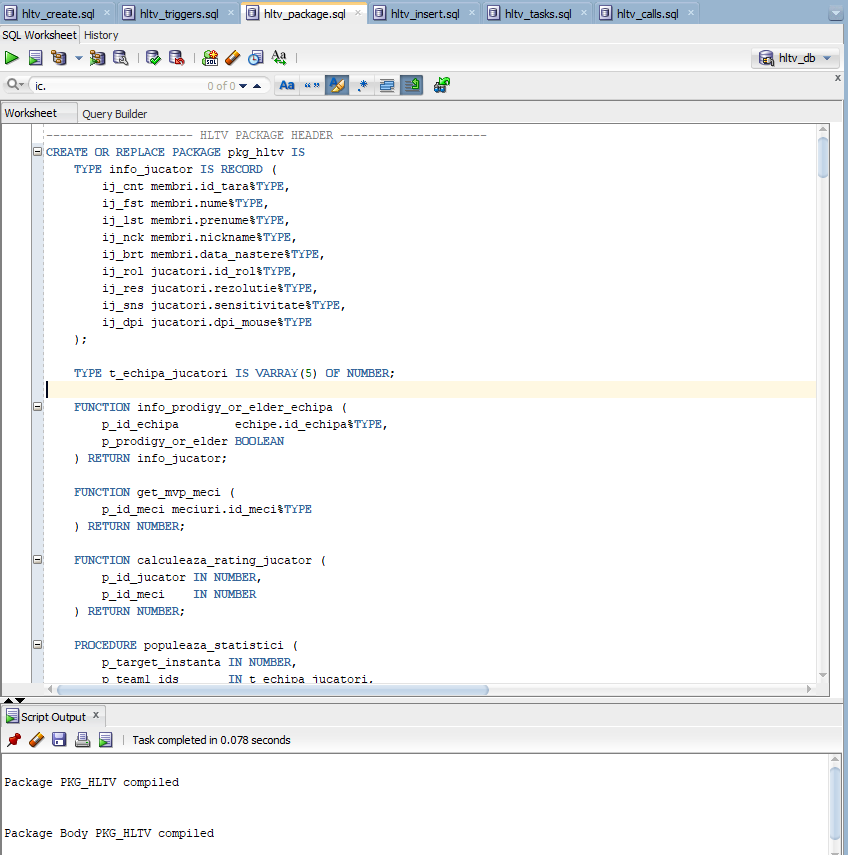
\includegraphics[width=\linewidth]{resources/hltv_package_script.png}
        \label{fig:hltv_package_script}
    \end{subfigure}
    \hfill
    \begin{subfigure}[b]{0.45\textwidth}
        \centering
        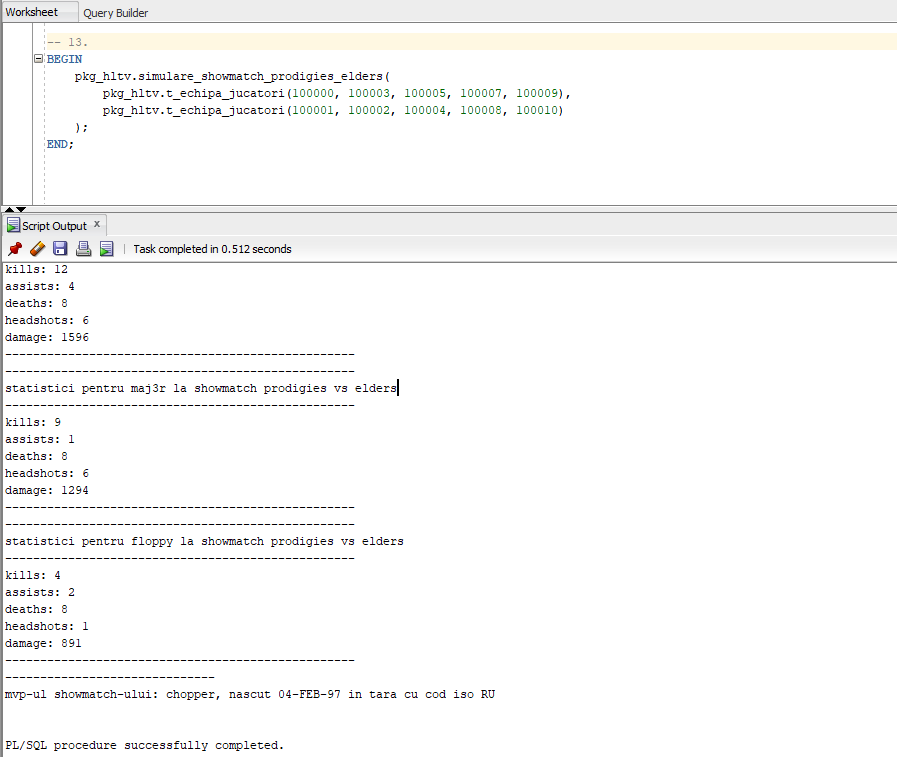
\includegraphics[width=\linewidth]{resources/output_task13.png}
        \label{fig:output_task13}
    \end{subfigure}
    \caption{Pachetul Compilat Corect și Exemplu de Apel de Procedură}
\end{figure}

\end{document}
